\documentclass[pdflatex,sn-basic]{sn-jnl}
\usepackage{graphicx,amsmath,amssymb,bm,booktabs,adjustbox,longtable,mathtools,enumitem}
\newcommand{\LABone}{LAB$_1$}
\newcommand{\LABtwo}{LAB$_2$}
\newcommand{\LABthree}{LAB$_3$}
\newcommand{\LAB}{LAB$_1$--LAB$_3$}
\newcommand{\StdTableFont}{\footnotesize}
\newcommand{\CohortN}{278}
\newcommand{\CohortMaleN}{128}
\newcommand{\CohortFemaleN}{150}
\newcommand{\CohortNoSwapN}{204}
\newcommand{\CohortSwapN}{74}
\newcommand{\ClusterMemberN}{152}
\newcommand{\ClusterMaleN}{90}
\newcommand{\ClusterFemaleN}{62}
\newcommand{\ClusterNoSwapN}{95}
\newcommand{\ClusterSwapN}{57}
\newcommand{\RankNineNo}{0.454}
\newcommand{\RankNineYes}{0.139}
\newcommand{\RankNineDifference}{-0.315}
\newcommand{\RankNineLow}{-0.360}
\newcommand{\RankNineHigh}{-0.262}
\newcommand{\RankNineRatio}{0.31}
\newcommand{\RankNinePval}{2.66e-23}
\newcommand{\RankNinePformatted}{2.7 \times 10^{-23}}
\newcommand{\RankNineRankBiserial}{-0.97}
\newcommand{\RankTenNo}{0.163}
\newcommand{\RankTenYes}{0.436}
\newcommand{\RankTenDifference}{0.273}
\newcommand{\RankTenLow}{0.225}
\newcommand{\RankTenHigh}{0.335}
\newcommand{\RankTenRatio}{2.68}
\newcommand{\RankTenPval}{1.70e-22}
\newcommand{\RankTenPformatted}{1.7 \times 10^{-22}}
\newcommand{\RankTenRankBiserial}{0.95}
\newcommand{\ScalarAPNo}{0.551}
\newcommand{\ScalarAPYes}{0.525}
\newcommand{\ScalarAPDifference}{-0.026}
\newcommand{\ScalarAPLow}{-0.084}
\newcommand{\ScalarAPHigh}{0.015}
\newcommand{\ScalarAPRatio}{0.95}
\newcommand{\ScalarAPPval}{3.03e-02}
\newcommand{\ScalarAPPformatted}{0.030}
\newcommand{\ScalarAPRankBiserial}{-0.21}
\newcommand{\PairAPNo}{0.077}
\newcommand{\PairAPYes}{0.075}
\newcommand{\PairAPDifference}{-0.002}
\newcommand{\PairAPLow}{-0.020}
\newcommand{\PairAPHigh}{0.012}
\newcommand{\PairAPRatio}{0.98}
\newcommand{\PairAPPval}{8.40e-01}
\newcommand{\PairAPPformatted}{0.840}
\newcommand{\PairAPRankBiserial}{-0.02}
\newcommand{\CohortRankNineNo}{0.458}
\newcommand{\CohortRankNineYes}{0.139}
\newcommand{\CohortRankNineDifference}{-0.319}
\newcommand{\CohortRankNineLow}{-0.355}
\newcommand{\CohortRankNineHigh}{-0.284}
\newcommand{\CohortRankNineRatio}{0.30}
\newcommand{\CohortRankNinePval}{9.73e-34}
\newcommand{\CohortRankNinePformatted}{9.7 \times 10^{-34}}
\newcommand{\CohortRankNineRankBiserial}{-0.95}
\newcommand{\CohortRankTenNo}{0.140}
\newcommand{\CohortRankTenYes}{0.441}
\newcommand{\CohortRankTenDifference}{0.301}
\newcommand{\CohortRankTenLow}{0.259}
\newcommand{\CohortRankTenHigh}{0.354}
\newcommand{\CohortRankTenRatio}{3.14}
\newcommand{\CohortRankTenPval}{4.26e-34}
\newcommand{\CohortRankTenPformatted}{4.3 \times 10^{-34}}
\newcommand{\CohortRankTenRankBiserial}{0.96}
\newcommand{\CohortScalarAPNo}{0.532}
\newcommand{\CohortScalarAPYes}{0.526}
\newcommand{\CohortScalarAPDifference}{-0.006}
\newcommand{\CohortScalarAPLow}{-0.048}
\newcommand{\CohortScalarAPHigh}{0.019}
\newcommand{\CohortScalarAPRatio}{0.99}
\newcommand{\CohortScalarAPPval}{1.06e-01}
\newcommand{\CohortScalarAPPformatted}{0.106}
\newcommand{\CohortScalarAPRankBiserial}{-0.13}
\newcommand{\CohortPairAPNo}{0.081}
\newcommand{\CohortPairAPYes}{0.076}
\newcommand{\CohortPairAPDifference}{-0.005}
\newcommand{\CohortPairAPLow}{-0.016}
\newcommand{\CohortPairAPHigh}{0.011}
\newcommand{\CohortPairAPRatio}{0.94}
\newcommand{\CohortPairAPPval}{7.80e-01}
\newcommand{\CohortPairAPPformatted}{0.780}
\newcommand{\CohortPairAPRankBiserial}{0.02}
\newcommand{\PrevalenceFiveSix}{33.8}
\newcommand{\PrevalenceNineTen}{54.7}
\newcommand{\PrevalenceTwelveThirteen}{28.1}
\newcommand{\PrevalenceTwelveFifteen}{41.7}
\newcommand{\PrevalenceFourteenFifteen}{25.2}
\newcommand{\BlockFiveSixAP}{0.33}
\newcommand{\BlockFiveSixML}{0.09}
\newcommand{\BlockFiveSixBIS}{0.95}
\newcommand{\BlockFiveSixBIT}{1.48}
\newcommand{\BlockFiveSixOUTLETAP}{0.50}
\newcommand{\BlockNineTenAP}{0.54}
\newcommand{\BlockNineTenML}{1.05}
\newcommand{\BlockNineTenBIS}{1.20}
\newcommand{\BlockNineTenBIT}{1.55}
\newcommand{\BlockNineTenOUTLETAP}{1.28}
\newcommand{\TotalPolyDOFs}{30}
\newcommand{\RigidDOFs}{6}
\newcommand{\NonrigidDOFs}{24}
\newcommand{\GramConditionNumber}{20.98}
\newcommand{\DesignConditionNumber}{4.58}
\newcommand{\CartilageEffectiveModulus}{1.0}

\newcommand{\StdTableInput}[1]{\begingroup\setlength{\tabcolsep}{4pt}\resizebox{\linewidth}{!}{\input{#1}}\endgroup}
\newcommand{\DetailTableInput}[1]{\begingroup\footnotesize\setlength{\tabcolsep}{4pt}\renewcommand{\arraystretch}{1.05}\noindent\centering\begin{adjustbox}{max width=\linewidth}\input{#1}\end{adjustbox}\par\endgroup}
\geometry{reset,a4paper,left=18mm,right=18mm,top=22mm,bottom=22mm}
\hfuzz=0pt
\usepackage{placeins}
\raggedbottom
\renewcommand{\dbltopfraction}{0.95}
\renewcommand{\textfraction}{0.05}
\setlength{\emergencystretch}{2em}
\begin{document}
\title[Pelvic deformation subspaces]{Comparing deformation subspaces across anatomical variability: a population finite-element study of the human pelvis}
\author[1,2]{\fnm{Petr} \sur{Heny\v{s}}}
\author[5]{\fnm{Michal} \sur{Kucha\v{r}}}
\author[5]{\fnm{Alexander} \sur{Mor\'{a}vek}}
\author*[2,3,4]{\fnm{Niels} \sur{Hammer}}\email{niels.hammer@medunigraz.at}
\affil[1]{\orgdiv{Institute of New Technologies and Applied Informatics, Faculty of Mechatronics, Informatics and Interdisciplinary Studies}, \orgname{Technical University of Liberec}, \orgaddress{\city{Liberec}, \country{Czech Republic}}}
\affil[2]{\orgdiv{Division of Macroscopic and Clinical Anatomy, Gottfried Schatz Research Center}, \orgname{Medical University of Graz}, \orgaddress{\city{Graz}, \country{Austria}}}
\affil[3]{\orgdiv{Department of Orthopedic and Trauma Surgery}, \orgname{University of Leipzig}, \orgaddress{\city{Leipzig}, \country{Germany}}}
\affil[4]{\orgdiv{Division of Biomechatronics}, \orgname{Fraunhofer Institute for Machine Tools and Forming Technology IWU}, \orgaddress{\city{Chemnitz and Dresden}, \country{Germany}}}
\affil[5]{\orgdiv{Department of Anatomy, Faculty of Medicine in Hradec Kr\'{a}lov\'{e}}, \orgname{Charles University}, \orgaddress{\city{Hradec Kr\'{a}lov\'{e}}, \country{Czech Republic}}}
\abstract{Comparing deformation modes across subject-specific finite-element models requires distinguishing changes in mechanical behaviour from changes in spectral ordering. We investigated this distinction in 278 computed-tomography-derived pelvic models with individual geometry and bone elasticity on a shared reference domain. The 15 lowest linearised stiffness modes were compared using spectral gaps, modal assignment, principal angles, anatomical diameter functionals, and modal strain-energy fractions under standing and internal-ring expansion loads. Modes 1--3 formed a well-separated, order-stable group with label-exchange rates below 0.4\%. A recurrent rank 9--10 cluster occurred in \PrevalenceNineTen\% of subjects. Within this cluster, median anteroposterior inlet coupling assigned to rank 9 decreased from 0.454 to 0.139 mm/mm between subjects without and with label exchange, whereas the corresponding subspace capacity changed from 0.551 to 0.525 mm/mm. Thus, the approximately 69\% difference at one rank greatly exceeded the approximately 5\% difference at the subspace level. Standing primarily recruited low-rank modes, whereas internal-ring expansion preferentially recruited the 9--10 block. An exploratory first-order material sensitivity analysis and a minimal analytical model contextualised the separation between rank instability and subspace-level deformation capacity. These findings support comparing compact modal subspaces when spectral crowding makes individual ranks unreliable. The framework distinguishes representation changes from changes in anatomical coupling within a linearised pelvic model. Expansion loads do not predict childbirth outcomes.}
\keywords{Population biomechanics, Pelvic mechanics, Finite-element modelling, Modal analysis, Anatomical variability, Invariant subspaces}
\maketitle
\clearpage
\section{Introduction}\label{sec:introduction}
The human pelvis transfers loads between the trunk and lower limbs while surrounding a canal whose dimensions have anatomical and obstetric significance. Its mechanical behaviour depends on the geometry and material distribution of the bones together with the sacroiliac joints, pubic symphysis, and ligamentous restraints. Accounts of sacroiliac load transfer emphasise this interaction between structural arrangement and stabilising tissues~\citep{Snijders1993,Vleeming2012}. Variation in pelvic form therefore raises a mechanical question beyond the description of shape: do anatomically different pelves retain comparable deformation pathways, and how are those pathways recruited by different loads? This question is relevant to understanding the relationship between pelvic form, load transmission, and canal deformation~\citep{Gruss2015}, even when the available models address only the initial elastic response.

Population modelling is necessary because a representative geometry cannot establish how mechanical behaviour varies among individuals. More generally, average model inputs need not produce an average biomechanical response~\citep{CookRobertson2016}. Population approaches have consequently become an explicit direction in computational musculoskeletal research~\citep{Fernandez2020Population}. For the pelvis, \citet{Arand2019PelvicShape} used CT-derived statistical modelling to characterise variation in pelvic-ring anatomy. Such models describe the distribution of geometry, but their principal components maximise geometric variance rather than identify mechanically compliant directions. A statistical shape mode and an elastic deformation mode thus answer different questions. Connecting anatomical variability to mechanics requires constitutive information, joint representation, and specified boundary conditions in addition to geometric correspondence.

CT-derived finite-element (FE) studies already provide substantial evidence for the importance of these factors. \citet{Salo2017PelvicStrain} compared pelvic strains across gait configurations in a validated cohort of five specimen-specific models. Their study demonstrates a route from individual anatomy to load-dependent strain predictions and documents variability between specimens. At the level of pelvic restraints, \citet{Henys2022Ligaments} examined how the sacrospinous and sacrotuberous ligaments influence pelvic kinematics and load redistribution. More recently, \citet{Chen2026PelvicModel} combined statistical shape modelling with musculoskeletal analysis to estimate sacroiliac and pubic joint reaction forces in females during standing and walking tasks. These studies establish relevant precedents for personalised pelvic mechanics. They also motivate a complementary question: which features of the available deformation repertoire remain comparable when both anatomy and the applied load differ?

Spectral analysis offers one way to organise that repertoire. Instead of describing the response to only one prescribed force pattern, a stiffness eigenproblem identifies deformation directions that can be combined to describe responses within a retained modal space. Pelvic modal analysis itself is established. \citet{HenysCapek2019Modal} investigated convergence and experimental validation of a CT-derived composite pelvic-bone model. A more direct antecedent is the study by \citet{Henys2021Eigenmetric}, which derived skeletal mechanical metrics from stiffness-matrix spectra and applied them to pelvic bones, relating these descriptors to anthropometric measurements and sex. That work established the value of spectral information beyond geometric measurements alone. It also left a consequential issue for population interpretation: an ordered eigenpair is a numerical descriptor, but its rank does not establish that its deformation pattern has the same anatomical meaning in every subject.

This issue becomes acute in crowded spectral regions. When neighbouring eigenvalues approach each other, changes in model parameters can produce marked changes in eigenvectors and their correspondence to reference patterns. Eigenvalue veering and mode localisation are well-established phenomena in structural mechanics~\citep{Pierre1988,ManconiMace2017}. For clustered spectra, \citet{GhoshGhanem2012} explicitly developed an invariant-subspace approach to stochastic eigenproblems, tracking the space spanned by neighbouring modes rather than requiring each eigenvector to remain individually identifiable. Thus, neither the spectral description of pelvic mechanics nor the use of subspaces for clustered eigenvalues is introduced here. The biomechanical question is what this distinction changes when interpreting anatomical deformation across a pelvic population.

For example, one eigenvector may strongly increase an inlet diameter in one subject, while a neighbouring eigenvector carries much of that displacement pattern in another. Comparing the same rank alone could then suggest a loss of inlet-opening capability even though a similar deformation remains available through a different combination of the two modes. Conversely, proximity of eigenvalues does not guarantee that an anatomical capacity is preserved. A clustered subspace can itself change with anatomy, and its coupling to a specific diameter can change even when its dimension is unchanged. A useful comparison must therefore assess spectral separation, correspondence of the spanned spaces, and anatomically defined observables together. Basis invariance removes dependence on the coordinates chosen within one space; preservation across subjects remains a hypothesis to test.

Anatomical observables make this distinction interpretable beyond numerical stability. Here, inlet and outlet diameter changes link displacement fields to recognisable pelvic dimensions. Maximising a diameter change within a modal subspace at a prescribed maximum nodal displacement measures the kinematic capacity available in that space. This quantity differs from compliance per unit force: a pathway can permit a particular diameter change without being strongly excited by a given load. Modal strain-energy decomposition provides the complementary assessment of recruitment under controlled loading. Considering both quantities allows us to ask whether standing and internal-ring expansion access different parts of the deformation repertoire, rather than inferring load-bearing function from mode shape alone.

Resolving this ambiguity matters whenever modal descriptors are used to compare individuals or groups. Before a difference at one rank is attributed to anatomy, sex, or material distribution, it is necessary to determine whether the compared modes retain correspondence. It also matters for the interpretation of reduced models: retaining a compact deformation space can be more meaningful than selecting individually labelled modes whose identities vary among subjects. These are immediate methodological uses of the present analysis. The broader biological motivation is to determine whether variation in pelvic form accompanies a reorganisation of mechanical pathways or a change in the anatomical deformation they can support. A linear elastic model can address the initial structural component of that question, while leaving physiological adaptation and actual childbirth mechanics unresolved.

Here, we analyse 278 CT-derived pelvic FE models using standardised geometries from BoneDat~\citep{HenyssKuchar2025BoneDat}, subject-specific bone elasticity, and a shared reference domain. We combine spectral gaps and modal assignment with principal-angle comparisons, basis-invariant anatomical capacities, and static load decomposition. We test three linked propositions: that well-separated low-rank modes retain correspondence across the cohort; that anatomical capacity within recurrent clustered subspaces varies less with mode-exchange status than coupling assigned to individual ranks; and that standing and internal-ring expansion recruit different spectral regions. Material-sensitivity analyses and a minimal analytical model contextualise these comparisons. The contribution is a population-level connection between spectral correspondence, anatomically defined deformation capacity, and load recruitment in the pelvic ring. The inferred rank groups describe this model family; the expansion loads are controlled mechanical probes rather than simulations of labour.

\section{Materials and methods}
\label{sec:methods}

The Methods below state the computational framework in self-contained form.
The core objects are (i)~a pullback-assembled linear-elasticity problem on a shared reference domain, (ii)~a subject-specific generalised eigenproblem, (iii)~a cross-subject pairing on a common mass metric, (iv)~a gap-based detector for recurrent clustered regimes, (v)~invariant-subspace comparison via principal angles and the Grassmann distance, and (vi)~basis-invariant anatomical functionals that supply physically interpretable coordinates inside otherwise ambiguous clustered subspaces.
Wherever possible, we use notation that separates three distinct objects: the solver \emph{rank} index~$j$ (the $j$-th smallest eigenvalue for each subject), the paired \emph{reference} label $i = \pi_s^{-1}(j)$ (a cross-subject identifier via inverse assignment), and the \emph{anatomical} functional~$\ell$ (a linear observable defined on the template mesh).


\subsection{Cohort and common-reference geometry}
\label{sec:cohort}

We analysed a precomputed set of $N{=}278$ CT-derived pelvic finite-element models assembled on a common reference domain ($n_F{=}150$, $n_M{=}128$; age 16--91~yr, mean $54\pm19$).
No new cohort was recruited.
The source repository provides standardised pelvic geometries suitable for in silico analysis~\citep{HenyssKuchar2025BoneDat}.
The reference pelvic domain $\Omega_{\rm ref}$ was discretized using a conforming volumetric mesh comprising $166\,808$ linear four-node tetrahedral elements (Lagrange $P_1$, $48\,291$ nodes, totaling $144\,873$ displacement degrees of freedom), with conforming interfaces between the bony segments (sacrum, left and right ossa coxae) and the joint cartilage domains (bilateral sacroiliac articular cartilage and the pubic symphysis disc).
A nonrigid volumetric registration $\chi_s: \Omega_{\rm ref}\to\Omega_s$ with deformation gradient $F_s(X)=\nabla_X\chi_s(X)$ and Jacobian $J_s=\det F_s$ maps the template domain $\Omega_{\rm ref}$ onto each subject domain $\Omega_s$.
The registration was obtained by radial-basis-function interpolation.
The registered geometries share anatomical correspondence, but size variation remains in the archived cohort. The primary analysis uses stored solver-order spectra without the separate post-hoc eigenvalue scale adjustment; isotropic size is examined as a covariate in the allometric analysis.
Fig.~\ref{fig:model-setup} summarises the anatomical dimensions, ligament representation, and boundary-condition layout used to define the pelvic models analysed here.




\begin{figure}[!t]
\centering
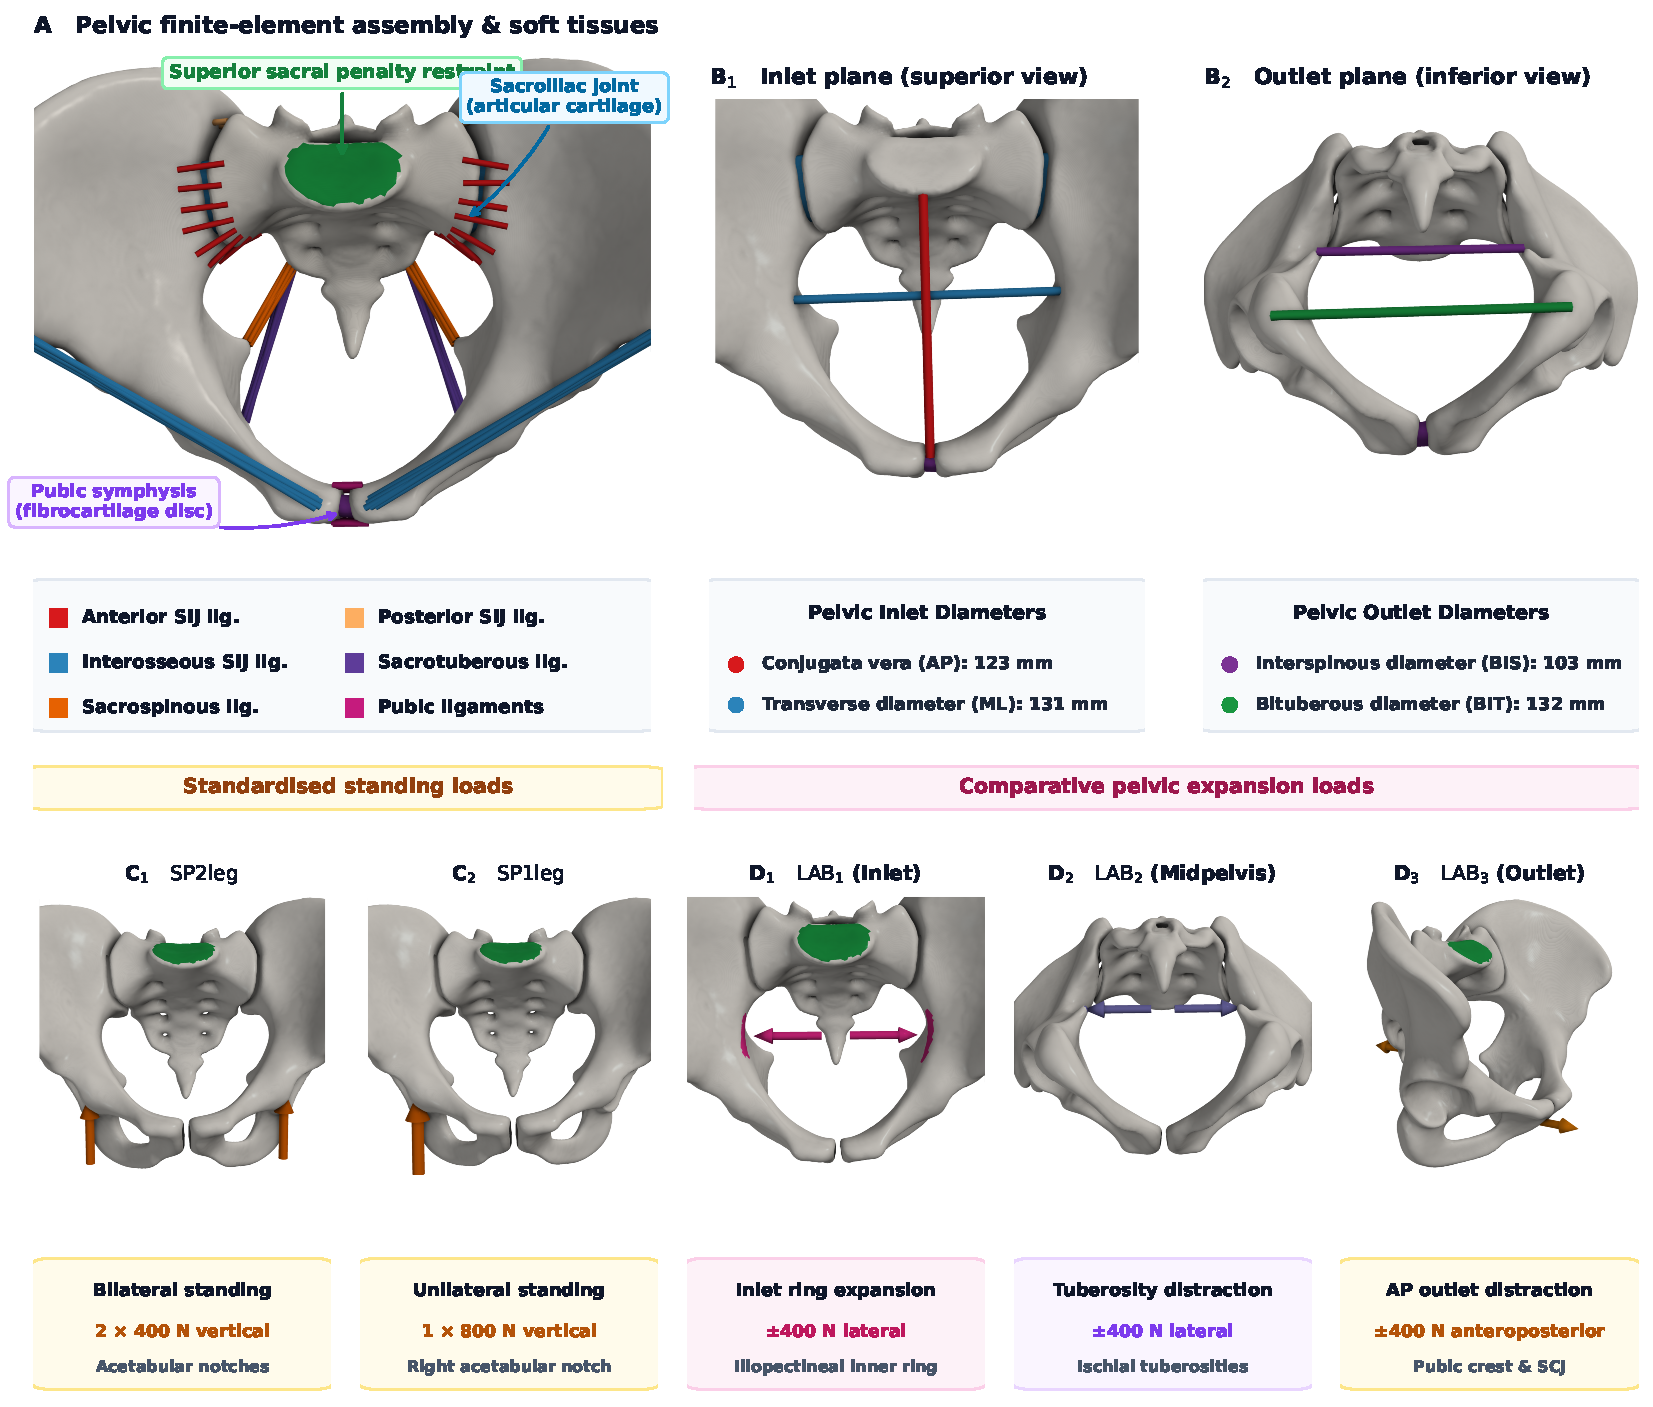
\includegraphics[width=\textwidth]{Fig1.pdf}
\caption{Pelvic model and standardised loading. \textbf{(A)} Bony segments, joint cartilage, ligament bundles, and superior sacral restraint. \textbf{(B)} Inlet and outlet diameter definitions on the reference anatomy. \textbf{(C)} Two-leg and one-leg standing loads. \textbf{(D)} Comparative internal-ring expansion, ischial distraction, and anteroposterior outlet distraction loads (\LAB). Each traction is normalised to the prescribed resultant across subjects. Expansion loads probe linear structural response and do not represent successive simulated stages of labour}
\label{fig:model-setup}
\end{figure}

\subsection{Pullback-assembled linear elasticity on a common reference domain}
\label{sec:pullback}

Let $\Omega_{\rm ref}\subset\mathbb R^3$ be the template domain and $\Omega_s$ the subject domain, related by a fixed volumetric registration $x=\chi_s(X)$ with deformation gradient $F_s(X)=\nabla_X\chi_s(X)$ and local Jacobian $J_s(X)=\det F_s$.
Writing $\chi_s(X)=X+\varphi_s(X)$, so $F_s=I+\nabla_X\varphi_s$, small-strain linear elasticity is solved on $\Omega_s$ but integrated on $\Omega_{\rm ref}$ through the standard change of variables~\citep{MarsdenHughes1983,BonetWood1997}.
For trial and test fields $\widehat{\mathbf u},\widehat{\mathbf v}\in V\subset[H^1(\Omega_{\rm ref})]^3$, the physical strain tensor at $x=\chi_s(X)$ is
\begin{equation}
\begin{gathered}
\bm\varepsilon_x(\mathbf u)=\mathrm{sym}(\nabla_x \mathbf u)=\mathrm{sym}\!\big(\nabla_X \widehat{\mathbf u}\,F_s^{-1}\big),
\\
\bm\sigma_x=C_{\rm phys}(x):\bm\varepsilon_x(\mathbf u),
\end{gathered}
\end{equation}
and the pullback-assembled elastic bilinear form reads
\begin{equation}
a(\widehat{\mathbf u},\widehat{\mathbf v})
=\int_{\Omega_{\rm ref}}\!\Big[C_{\rm phys}\!\big(\chi_s(X)\big):\mathrm{sym}\!\big(\nabla_X \widehat{\mathbf u}\,F_s^{-1}\big)\Big]
:\mathrm{sym}\!\big(\nabla_X \widehat{\mathbf v}\,F_s^{-1}\big)\,J_s\,\mathrm dX.
\label{eq:pullback-bilinear}
\end{equation}
Here $F_s$ and $J_s$ arise only from the fixed image registration; no finite-strain mechanics is implied.
The mass bilinear form inherits the geometric volume factor,
\begin{equation}
m(\widehat{\mathbf u},\widehat{\mathbf v})
=\int_{\Omega_{\rm ref}} J_s(X)\,\widehat{\mathbf u}\cdot\widehat{\mathbf v}\,\mathrm dX,
\label{eq:mass-subject}
\end{equation}
defining an $L^2$ volume inner product weighted by local volumetric dilation rather than physical dynamic mass density.
The resulting generalised eigenvalues $\lambda_k = \boldsymbol\phi_k^\top K_s \boldsymbol\phi_k / (\boldsymbol\phi_k^\top M_s \boldsymbol\phi_k)$ are stiffness-spectrum descriptors in a volume metric. With coordinates in mm and modulus in MPa they have units N/mm$^4$; their reciprocals have units mm$^4$/N and are not point compliances. They are not physical resonance frequencies because $M_s$ does not include mass density.
The \emph{unmapped} reference mass matrix $M_{\rm ref}^{0}$ is obtained from~\eqref{eq:mass-subject} with $J\equiv 1$ and provides a shared, registration-independent inner product across subjects.


\noindent\textbf{Material model.}
The physical elasticity tensor $C_{\rm phys}(x)$ is isotropic and heterogeneous.
For bone, the CT-derived hydroxyapatite density $\rho(x)$ is converted to ash density $\rho_{\mathrm{ash}}=(\rho+0.09)/1.14$ and mapped to a Young's modulus $E(x)$ using an implemented piecewise approximation motivated by Keller~\citep{Keller1994},
\begin{equation}
\begin{gathered}
E(x)=\begin{cases}
2398\,\mathrm{MPa}, & \rho_{\mathrm{ash}}(x)\le 0.486,\\[2pt]
\alpha\,\rho_{\mathrm{ash}}(x)^{\beta}, & \rho_{\mathrm{ash}}(x)>0.486,
\end{cases}
\\
 \alpha=10\,200,\ \beta=2.0,
\label{eq:keller}
\end{gathered}
\end{equation}
with Poisson's ratio $\nu=0.3$. Negative input densities are clipped to zero. The law is applied at source points, after which the resulting modulus is interpolated to FE cells using RBF interpolation (smoothing parameter 50, ten neighbours). The constant low-density branch and the exponent 2.0 are modelling choices rather than an exact reproduction of the cited regression. Density--modulus calibration depends on anatomical site~\citep{Morgan2003Trabecular} and was not performed individually for this cohort.
Cartilage (sacroiliac joints and pubic symphysis) is homogeneous linear elastic with $E=1.0$\,MPa and $\nu=0.45$.
These parameters are prescribed effective values. General accounts of bone adaptation~\citep{Frost1987,Huiskes1987} and pelvic joint mechanics~\citep{Snijders1993,Vleeming2012,Goode2008} provide context but do not validate their numerical values.

\noindent\textbf{Ligaments in pullback coordinates.}
Ligament families are represented as polyline bundles mapped from template nodes $X_i$ to physical points $x_i=\chi_s(X_i)$.
For each segment $(X_i,X_j)$ define the physical unit tangent $\mathbf e=(x_j-x_i)/\|x_j-x_i\|$ and length $L=\|x_j-x_i\|$.
The total bundle stiffness and pretension are distributed across $N_{\rm seg}$ segments, yielding per-segment $k_{\rm seg}=K_{\rm bundle}/N_{\rm seg}$ and $T_{\rm seg}=T_{\rm bundle}/N_{\rm seg}$.
Each segment contributes an axial stiffness block
\begin{equation}
W=k_{\rm seg}\,(\mathbf e\mathbf e^\top),\qquad
K^{\rm ax}_{ij}=\begin{bmatrix} +W & -W\\ -W & +W\end{bmatrix},
\end{equation}
and, in the presence of pretension $T_{\rm seg}\ge 0$, a geometric (prestress) stiffness
\begin{equation}
W_g=\tfrac{T_{\rm seg}}{L}\big(I-\mathbf e\mathbf e^\top\big),\qquad K^{\rm geo}_{ij}=\begin{bmatrix}W_g&-W_g\\-W_g&W_g\end{bmatrix}\succeq0,
\label{eq:kgeo}
\end{equation}
together with paired nodal forces $\pm T_{\rm seg}\mathbf e$ on the right-hand side.
The assembled linear stiffness, including prescribed ligament prestress, is
\begin{equation}
K_s=K_{\rm elas,s}+K_{\rm lig,s}+K^{\rm geo}_s(T)+K_{\Gamma,s},\qquad
f=f_{\rm ext}+f_{\rm pret}(T),
\label{eq:K-assembled}
\end{equation}
where geometric stiffness $K^{\rm geo}_s(T)$ incorporates the stabilizing effect of initial ligament pretension $T$. This is a linear approximation with prescribed prestress; a geometrically nonlinear equilibrated prestressed configuration was not established.
The term $K_{\Gamma,s}$ implements Dirichlet penalties on the restrained superior sacral facet $\Gamma_{\rm ref}$,
$a_\Gamma(\widehat{\mathbf u},\widehat{\mathbf v})=\gamma\int_{\Gamma_{\rm ref}} \widehat{\mathbf u}\cdot\widehat{\mathbf v}\,J_{\Gamma,s}\,\mathrm dS_X$ with $J_{\Gamma,s}=J_s\|F_s^{-T}N\|$, using a fixed penalty parameter $\gamma = 10^6\,\mathrm{N/mm^3}$ prescribed directly without element-size or modulus scaling.
A decade sweep of $\gamma$ across $[10^5, 10^7]\,\mathrm{N/mm^3}$ left the reported cluster classification and modal subspace capacities unchanged.

\noindent\textbf{Force-controlled loading.}
Neumann terms are pulled back to $\Gamma_{\rm ref}$ so that physical resultants are invariant under $\chi_s$:
\begin{equation}
\int_{\Gamma_s}\mathbf t_{\rm phys}\!\cdot\!\mathbf v\,\mathrm dS_x
=\int_{\Gamma_{\rm ref}} J_{\Gamma,s}(X)\,\mathbf t_{\rm phys}(\chi_s(X))\cdot\widehat{\mathbf v}(X)\,\mathrm dS_X.
\label{eq:neumann-pullback}
\end{equation}
All load cases in this study are defined by a total force $\mathbf F$ on a tagged physical region; the applied traction is $\mathbf t_{\rm phys}=\mathbf F/A_{\rm phys}$ with $A_{\rm phys}=\int_{\Gamma_{\rm ref}}J_{\Gamma,s}\,\mathrm dS_X$, so that $\int_{\Gamma_s}\mathbf t_{\rm phys}\,\mathrm dS_x=\mathbf F$ for every subject.

\subsection{Standardised load cases}
\label{sec:loading}

Loads were applied as force-controlled Neumann tractions via~\eqref{eq:neumann-pullback} so that every subject experienced the same integrated force vector regardless of physical surface area.
Two standing cases were considered: symmetric two-leg stance (SP2leg; $400$\,N per acetabulum, $+$CC) and one-leg stance (SP1leg; $800$\,N on the stance acetabulum, $+$CC).
The 400\,N per hip and 800\,N one-leg magnitudes are prescribed comparative loads. The cited in-vivo hip-contact forces provide context for physiological loading but do not validate these particular traction fields~\citep{Bergmann2001JBiomech,Kutzner2016PLOS}.
Three proxy load cases probed parturition-relevant routing without modelling contact mechanics: \LABone\ applied bilateral mediolateral internal ring expansion forces ($\pm 400$\,N outward), \LABtwo\ applied bilateral ischial-tuberosity distraction ($\pm 400$\,N), and \LABthree\ applied anteroposterior outlet distraction between the pubis insertion ($-$AP, $400$\,N) and the sacrococcygeal joint ($+$AP, $400$\,N).
These loads act as standardized comparative probes of pelvic structural compliance rather than clinical simulations of labour~\citep{ChenGrimm2021,Almeida2024Uterus}.
Static finite-element solutions solve the linear equilibrium equation $K_s \mathbf u = \mathbf b$ with
\begin{equation}
\mathbf b = \mathbf f_{\rm ext} + \mathbf f_{\rm pret}
\label{eq:total-load-vector}
\end{equation}
for the primary total-response analysis, where $\mathbf f_{\rm pret}$ represents baseline ligament pretension ($20$\,N per ligament bundle) and $\mathbf f_{\rm ext}$ represents external load.
Primary cohort-wide modal strain-energy fractions (Section~\ref{sec:load-results}; Table~\ref{tab:dominant-sets}) are computed directly from these total displacement fields $\mathbf u$.
By linearity, total displacement decomposes as $\mathbf u = \mathbf u_{\rm pret} + \delta\mathbf u_{\rm ext}$, where $\delta\mathbf u_{\rm ext} = K_s^{-1}\mathbf f_{\rm ext}$ is the incremental external load response.
Under external load scaling $\mathbf f_{\rm ext} \to c\mathbf f_{\rm ext}$, incremental displacements scale proportionally ($\delta\mathbf u_{\rm ext} \to c\,\delta\mathbf u_{\rm ext}$), such that modal expansion coefficients $q_i = \boldsymbol\phi_i^\top M_s \delta\mathbf u_{\rm ext}$ scale by $c$, modal energies $E_i = \frac{1}{2}\lambda_i q_i^2$ scale by $c^2$, and the normalized modal strain-energy fractions $f_i = E_i / \sum_j E_j$ of the incremental response are strictly scale-invariant.
To examine the effect of baseline pretension on routing, we compared archived total-response and incremental-response modal fractions in 18 subjects with complete stored incremental outputs. The top recruited mode agreed for all five loads in all 18 subjects. The maximum individual change in the 9--10 block fraction was 4.24 percentage points, while its mean change under \LABone\ was $+3.48$ percentage points. The smallest dominant set reaching 80\% of retained energy had the same size in all 18 standing cases and in 14 of 18 \LABone\ cases. This subset supports similar dominant routing but does not establish exact invariance across the full cohort.

\subsection{Generalised eigenproblem, rigid-mode filtering, and cross-subject pairing}
\label{sec:evp}

For each subject $s$ we assembled $(K_s,M_s)$ on $\Omega_{\rm ref}$ via~\eqref{eq:K-assembled} and~\eqref{eq:mass-subject} and solved the generalised eigenproblem
\begin{equation}
K_s\boldsymbol\phi_k=\lambda_k M_s\boldsymbol\phi_k,\qquad
\boldsymbol\phi_i^\top M_s \boldsymbol\phi_j=\delta_{ij},
\label{eq:gep}
\end{equation}
using a Krylov--Schur solver (SLEPc) with shift-invert spectral transform and MUMPS direct factorisation, extracting the $N_{\rm ev}=15$ lowest non-rigid eigenpairs.
Rigid modes (numerically $\lambda<10^{-8}$) were filtered.
For cross-subject comparison we used the mass-weighted modal assurance criterion on the shared reference metric,
\begin{equation}
\mathrm{MAC}_{M_0}(\mathbf x,\mathbf y)=
\frac{|\mathbf x^\top M_{\rm ref}^{0}\mathbf y|^2}
{(\mathbf x^\top M_{\rm ref}^{0}\mathbf x)(\mathbf y^\top M_{\rm ref}^{0}\mathbf y)}\in[0,1],
\label{eq:mac}
\end{equation}
and solved the Hungarian optimal-assignment problem on $-\mathrm{MAC}_{M_0}$ over the full $N_{\rm ev}\times N_{\rm ev}$ matrix~\citep{Kuhn1955Hungarian}, yielding an assignment bijection $\pi_s: \{1,\dots,N_{\rm ev}\} \to \{1,\dots,N_{\rm ev}\}$, where $\pi_s(i_{\rm ref}) = j_{\rm rank}$ maps reference identifier $i_{\rm ref}$ to its rank position in subject~$s$, and the inverse permutation $\pi_s^{-1}(j_{\rm rank}) = i_{\rm ref}$ assigns reference identity to each solver rank.
Entries with $\mathrm{MAC}_{M_0}<0.05$ were flagged as unpaired.
Rank index~$j$ (solver order) is required for gap statistics and cluster detection; the inverse assignment $\pi_s^{-1}(j)$ maps each solver mode back to its reference identity and is used only for anatomical interpretation, preserving the distinction between rank order and pathway identity emphasised in the Introduction.


\subsection{Spectral gap structure and clustered-regime detection}
\label{sec:gaps}

For each subject with ordered eigenvalues $\lambda_1\le\cdots\le\lambda_{N_{\rm ev}}$, relative consecutive gaps are
\begin{equation}
\mathrm{gap}_{\rm in}(i)=\frac{\lambda_{i+1}-\lambda_i}{\lambda_i},\qquad i=1,\ldots,N_{\rm ev}-1.
\label{eq:gap-in}
\end{equation}
A clustered regime $[i..j]$ is defined as the maximal contiguous rank block starting at~$i$ with internal gaps below threshold, $\mathrm{gap}_{\rm in}(k)<\varepsilon_{\rm in}$ for $k=i,\ldots,j-1$.
The threshold is set from data as the 25th percentile of the pooled $\mathrm{gap}_{\rm in}$ distribution across the cohort, yielding $\varepsilon_{\rm in}\approx 0.13$; sensitivity to the percentile choice is reported in Section~\ref{sec:details-D}.
External separation is quantified by
\begin{equation}
\mathrm{sep}_{\rm out}([i..j])=\min\!\left(\frac{\lambda_i-\lambda_{i-1}}{\lambda_i},\ \frac{\lambda_{j+1}-\lambda_j}{\lambda_j}\right),
\label{eq:sep-out}
\end{equation}
defined for interior clusters ($i > 1$ and $j < N_{\rm ev}$) where both adjacent neighbours exist. For boundary blocks reaching modal truncation (such as the 12--15 cluster with $N_{\rm ev}=15$), the upper neighbour is uncomputed and two-sided separation is formally undefined.
Exact mathematical multiplicity ($\lambda_i = \lambda_{i+1}$) was not observed under the operational numerical tolerance $\mathrm{gap}_{\rm in}\le\varepsilon_{\rm deg}=10^{-6}$ in any subject. No obvious spatial symmetry was identified that would enforce repeated eigenvalues, although accidental parameter-dependent crossings are not mathematically excluded; nonetheless, the regimes detected by~\eqref{eq:gap-in} are operational small-gap clusters in which perturbation sensitivity may be elevated~\citep{Pierre1988,ManconiMace2017}.

\subsection{Invariant subspaces: principal angles, Grassmann distance, and Procrustes alignment}
\label{sec:subspace-methods}

For each clustered rank block of dimension~$r$, the corresponding subject-specific subspace was represented by an $M_{\rm ref}^{0}$-orthonormal basis
\begin{equation}
Q_s\in\mathbb R^{n\times r},\qquad Q_s^\top M_{\rm ref}^{0}\,Q_s=I_r.
\end{equation}
With a fixed reference basis $Q_{\rm ref}$, define the overlap matrix
\begin{equation}
S=Q_{\rm ref}^\top M_{\rm ref}^{0}\,Q_s\in\mathbb R^{r\times r},\qquad S=U\Sigma V^\top,\qquad \cos\theta_k=\sigma_k(S),
\label{eq:overlap}
\end{equation}
with singular values $\sigma_k$ yielding the principal angles $\theta_k\in[0,\pi/2]$ between the two subspaces~\citep{BjorckGolub1973Angles}.
The Grassmann distance is
\begin{equation}
d_G(Q_{\rm ref},Q_s)=\|\boldsymbol\theta\|_2=\Big(\sum_{k=1}^{r}\theta_k^2\Big)^{1/2}.
\label{eq:grassmann}
\end{equation}
When a stable basis representation inside a clustered subspace is required, we apply an orthogonal Procrustes rotation~\citep{Schoenemann1966Procrustes},
\begin{equation}
\widetilde Q_s=Q_s\,(V U^\top),
\label{eq:procrustes}
\end{equation}
which minimises the $M_{\rm ref}^{0}$-weighted distance $\|Q_{\rm ref} - Q_s R\|_{M_{\rm ref}^0}$ over orthogonal matrices $R\in\mathrm O(r)$ while preserving the subspace $\mathrm{span}(Q_s)$.

Subspace comparisons use basis-invariant scalars derived below. Individual-rank couplings remain explicit comparators whose sensitivity to mode exchange is being tested.

\noindent\textbf{Degeneracy vs.\ near-degenerate mixing.}
Exact mathematical multiplicity requires $\lambda_i = \lambda_{i+1}$ (operationalized numerically as $\mathrm{gap}_{\rm in}(k)\le\varepsilon_{\rm deg}$ for all $k$ in the block, with $\varepsilon_{\rm deg}\ll\varepsilon_{\rm in}$); individual eigenvectors inside a degenerate subspace are then not unique, and any unitary rotation inside $\mathrm{span}(Q_s)$ is an equally valid basis.
When $\varepsilon_{\rm deg}<\mathrm{gap}_{\rm in}(k)<\varepsilon_{\rm in}$ the eigenvalues are close but distinct; each eigenvector is unique up to sign, yet small perturbations can rotate the internal basis substantially while the spanned subspace can be less sensitive if its external separation is sufficiently large relative to the perturbation. Neither a small internal gap nor label exchange alone proves preservation of anatomical coupling.

\subsection{Canonical anatomical functionals inside clustered subspaces}
\label{sec:canonical-methods}

To interpret clustered subspaces biologically, we use basis-invariant linear functionals defined by anatomical landmark pairs.
On the reference template mesh, five key obstetric and locomotor diameters are defined:
\begin{enumerate}[label=(\roman*)]
\item \textbf{AP inlet} ($s_{\rm AP}$): Promontory ($X_{\rm prom}$) to superior pubic symphysis ($X_{\rm pub}$), with unit direction $\mathbf e_{\rm AP} = (X_{\rm pub} - X_{\rm prom}) / \|X_{\rm pub} - X_{\rm prom}\|$;
\item \textbf{ML inlet} ($s_{\rm ML}$): Widest transverse diameter across left and right iliopectineal lines ($X_{\rm left}, X_{\rm right}$), with unit direction $\mathbf e_{\rm ML} = (X_{\rm right} - X_{\rm left}) / \|X_{\rm right} - X_{\rm left}\|$;
\item \textbf{Interspinous midpelvic diameter (BIS)} ($s_{\rm BIS}$): Left to right ischial spine ($X_{\rm sp,left}, X_{\rm sp,right}$), with unit direction $\mathbf e_{\rm BIS} = (X_{\rm sp,right} - X_{\rm sp,left}) / \|X_{\rm sp,right} - X_{\rm sp,left}\|$;
\item \textbf{Bituberous outlet} ($s_{\rm BIT}$): Left to right inferior ischial tuberosity ($X_{\rm tub,left}, X_{\rm tub,right}$), with unit direction $\mathbf e_{\rm BIT} = (X_{\rm tub,right} - X_{\rm tub,left}) / \|X_{\rm tub,right} - X_{\rm tub,left}\|$;
\item \textbf{AP outlet} ($s_{\rm OUTLETAP}$): Sacrococcygeal joint ($X_{\rm cocc}$) to inferior pubic symphysis ($X_{\rm pub,inf}$), with unit direction $\mathbf e_{\rm OUTAP} = (X_{\rm pub,inf} - X_{\rm cocc}) / \|X_{\rm pub,inf} - X_{\rm cocc}\|$.
\end{enumerate}
For each subject $s$, patient-specific landmark coordinates follow the registration mapping $X^s = X + \boldsymbol\varphi_s(X)$, and the resulting functional observable for a displacement field $\mathbf u$ is
\begin{equation}
\begin{gathered}
s_\ell^{(s)}(\mathbf u) = \mathbf e_\ell^{(s)\top}\! \big(\mathbf u(X_{\rm target}^s) - \mathbf u(X_{\rm origin}^s)\big) = \mathbf b_\ell^{(s)\top}\mathbf u, \\
 \ell \in \{\text{AP, ML, BIS, BIT, OUTLETAP}\},
\label{eq:functional-score}
\end{gathered}
\end{equation}
with measurement vectors $\mathbf b_\ell^{(s)}\in\mathbb R^n$ constructed using inverse-distance-squared weighting over the 32 nearest reference-mesh nodes at each template landmark. These weights remain fixed across subjects; the direction $\mathbf e_\ell^{(s)}$ is updated from RBF-mapped landmark positions. BIS measures the midpelvis between the ischial spines, whereas BIT measures the intertuberous outlet. The AP-outlet observable uses the sacrococcygeal landmark and is not a coccygeal-tip diameter.

\noindent\textbf{Basis-invariant max-nodal anatomical capacity.}
For any individual functional $\mathbf b_\ell^{(s)}$ and an orthonormal basis $Q_s \in \mathbb R^{n \times r}$ spanning a clustered subspace of dimension $r$ ($Q_s^\top M_{\rm ref}^0 Q_s = I_r$), every displacement in the subspace is parameterized by $\mathbf u = Q_s \boldsymbol\alpha$ with $\boldsymbol\alpha \in \mathbb R^r$.
The maximum anatomical diameter response per 1\,mm maximum nodal displacement is defined by the constrained max-nodal capacity:
\begin{equation}
\kappa_{\ell,\infty}(Q_s) = \max_{\boldsymbol\alpha \ne \mathbf 0} \frac{|\mathbf b_\ell^{(s)\top} Q_s \boldsymbol\alpha|}{\max_a \|(Q_s \boldsymbol\alpha)_a\|_2} = \max_{\boldsymbol\alpha} |\mathbf b_\ell^{(s)\top} Q_s \boldsymbol\alpha| \quad \text{s.t.} \quad \max_a \|(Q_s \boldsymbol\alpha)_a\|_2 \le 1,
\label{eq:single-functional-max-nodal}
\end{equation}
where $a$ indexes the finite-element mesh nodes and $\|(Q_s \boldsymbol\alpha)_a\|_2$ denotes the Euclidean displacement norm of node $a$.
Because both the numerator and the max-nodal constraint depend only on the physical displacement field $\mathbf u = Q_s \boldsymbol\alpha$, this quantity is strictly invariant under arbitrary internal orthogonal basis rotations $\widetilde Q_s = Q_s R$ with $R \in \mathrm O(r)$, since $\widetilde Q_s (R^\top \boldsymbol\alpha) = Q_s \boldsymbol\alpha$.
For $r=2$, the zero-homogeneity of the objective allows parameterization of $\boldsymbol\alpha$ by polar angle $\theta \in [0, \pi)$ with $\boldsymbol\alpha(\theta) = (\cos\theta, \sin\theta)^\top$, estimated from 90 angular samples followed by scalar refinement. For $r\ge3$, we solve the equivalent convex program $\max_{\boldsymbol\alpha} \mathbf c^\top\boldsymbol\alpha$ subject to $\|(Q_s\boldsymbol\alpha)_a\|_2\le1$ at every node, where $\mathbf c=Q_s^\top\mathbf b_\ell^{(s)}$; the sign symmetry removes the absolute value. Constraint generation starts with 16 nodes, solves each reduced problem with SLSQP and analytic Jacobians, adds the most violated mesh node, and terminates only when the full-mesh maximum squared norm is at most $1+10^{-8}$. The objective is linear and every constraint is convex, so a feasible stationary solution is a global optimum of the finite-dimensional problem up to numerical tolerance. Four independent full-constraint optimisations provide an additional check.
The optimal spatial displacement field $\boldsymbol\psi_\ell^{(s)} = Q_s \boldsymbol\alpha^* / \max_a \|(Q_s \boldsymbol\alpha^*)_a\|_2$ satisfies $\max_a \|\boldsymbol\psi_{\ell,a}^{(s)}\|_2 = 1.0$ exactly, and the resulting anatomical capacity $\kappa_{\ell,\infty}(Q_s) = |\mathbf b_\ell^{(s)\top}\boldsymbol\psi_\ell^{(s)}|$ has physical units of millimetres diameter change per millimetre maximum nodal displacement.

\noindent\textbf{Multivariate canonical decomposition.}
When joint coupling across a pair of measurement vectors $(\mathbf b_1^{(s)}, \mathbf b_2^{(s)})$ (e.g., AP and ML inlet, or BIS and BIT outlet) is examined, we assemble the covector matrix $B_s = [\mathbf b_1^{(s)}\ \ \mathbf b_2^{(s)}] \in \mathbb R^{n \times 2}$ and its subspace projection:
\begin{equation}
\begin{gathered}
C_s = Q_s^\top B_s = \big[Q_s^\top\mathbf b_1^{(s)}\ \ Q_s^\top\mathbf b_2^{(s)}\big] \in \mathbb R^{r \times 2}, \\
 C_s = U_s \Sigma_s V_s^\top,
\label{eq:canonical-proj}
\end{gathered}
\end{equation}
where the singular values $\sigma_1\ge\sigma_2$ describe joint coupling under the coefficient constraint $\|\boldsymbol\alpha\|_2=1$, equivalent to unit norm in $M_{\rm ref}^0$. They do not give maxima under the max-nodal displacement constraint.
The canonical displacement modes in physical space are $\boldsymbol\psi_k^{(s)} = Q_s U_s[:, k]$ ($k=1, 2$), with corresponding dual functionals in covector space $\widetilde{\mathbf b}_k^{(s)} = B_s V_s[:, k] = V_s[0, k]\mathbf b_1^{(s)} + V_s[1, k]\mathbf b_2^{(s)}$.
By construction, their action is exactly equal to the singular values: $\widetilde{\mathbf b}_k^{(s)\top}\boldsymbol\psi_k^{(s)} = \sigma_k$.
The singular-direction scores subsequently normalized by maximum nodal displacement are $\widehat s_k^{(s)} = \sigma_k / \max_a \|\boldsymbol\psi_{k,a}^{(s)}\|_2$.
Because $V_s \in \mathrm O(2)$ mixes the two anatomical axes, mode $\boldsymbol\psi_1^{(s)}$ is primary-dominant only when $|V_s[0, 0]| \ge |V_s[1, 0]|$; across the pelvic cohort, the first singular mode in the 9--10 subspace is predominantly aligned with the more strongly coupled transverse (ML) axis ($|V_s[1, 0]| > |V_s[0, 0]|$ in $99.6\%$ of subjects).
For unambiguous, axis-specific evaluation of anatomical opening without coordinate mixing, the basis-invariant single-functional capacity $\kappa_{\ell,\infty}(Q_s)$ (Eq.~\eqref{eq:single-functional-max-nodal}) serves as our primary quantitative metric, while joint-SVD scores provide complementary bivariate structure.

\subsection{Whole-pelvis deformation decomposition}\label{sec:mechanisms-methods}
To distinguish global ring kinematics from joint-localised strains, we decompose the reference displacement fields after removing infinitesimal rigid motion. The fractions below describe the explained squared displacement norm within a specified polynomial dictionary, not elastic energy. Synthetic checks, the reference-mode atlas, and complete profile tables are provided in Section~\ref{sec:details-E}.

\subsubsection{Joint strain and global ring kinematics}
The pelvic ring is a closed, doubly-curved structural biomechanical loop composed of three major bony segments (the sacrum and bilateral coxal bones) joined anteriorly at the pubic symphysis and posteriorly at the bilateral sacroiliac joints (SIJs).
In continuum mechanics, the standard approach to characterise modal kinematics would be to evaluate the infinitesimal Cauchy strain tensor field,
\begin{equation}
\boldsymbol\varepsilon(\mathbf u) = \tfrac{1}{2}\big(\nabla \mathbf u + \nabla \mathbf u^\top\big).
\label{eq:cauchy-strain}
\end{equation}
In the present quasi-static finite-element formulation, an effective joint modulus of $E_{\rm cartilage} = \CartilageEffectiveModulus\,\mathrm{MPa}$ is prescribed for the sacroiliac cartilage cleft and pubic symphysis disc.
This prescribed modulus represents compliant joint regions within the model, which are three to four orders of magnitude more compliant than cortical and trabecular bone ($E_{\rm bone} \sim 5\text{--}18\,\mathrm{GPa}$).
Under the generalised modal formulation, elastic deformation naturally channels into these narrow compliant interfaces.
Consequently, direct $L^2$-projection of the Cauchy strain field onto low-order polynomial strain templates leaves between 97\% and 99\% of the strain norm unexplained in the residual across all fifteen computed eigenmodes.
The intense local strain spikes in the millimeter-thin joint clefts completely overpower and conceal the systemic, ring-scale kinematics (such as whole-pelvis flaring, torsion, and inlet/outlet dilation).

A dictionary conditioned along only one anatomical axis did not describe coupled three-dimensional ring deformation adequately in the tested example.
For complex three-dimensional deformation pathways involving coupled out-of-plane flexure and transverse shearing (such as Mode~2), the tested one-axis dictionary left an 84\% residual. This reflects the scope of that descriptive basis and is not evidence that all beam approximations are unphysical.
To overcome both limitations, our framework evaluates the overall shape change across the entire three-dimensional pelvic continuum without anatomical partitioning and without imposing artificial 1D beam axes, removing infinitesimal rigid-body motion upfront before decomposing the remaining shape change into four canonical 3D polynomial deformation families.

\subsubsection{Continuum inner product and tetrahedral quadrature}
Let $\Omega \subset \mathbb{R}^3$ denote the reference pelvic continuum domain with volume $V = \int_\Omega \mathrm{d}V$.
The natural inner product on the displacement space $[L^2(\Omega)]^3$ weighted by volume is
\begin{equation}
\begin{gathered}
\langle \mathbf u, \mathbf v \rangle_V = \frac{1}{V} \int_\Omega \mathbf u(\mathbf x) \cdot \mathbf v(\mathbf x) \, \mathrm{d}V, \\
\|\mathbf u\|_V^2 = \langle \mathbf u, \mathbf u \rangle_V.
\label{eq:volume-inner-product}
\end{gathered}
\end{equation}
The continuous reference domain $\Omega$ is discretized into an unstructured tetrahedral mesh $\mathcal{T}_h = \{K_e\}_{e=1}^{N_e}$ using piecewise-linear ($P_1$) Lagrange continuous finite elements.
Within any tetrahedron $K$, a $P_1$ displacement field $\mathbf u_h(\mathbf x)$ is an affine vector function of position ($\mathbf u_h|_K \in \mathcal{P}_1(K)$).
When computing projections against quadratic deformation modes $\mathbf p_2 \in \mathcal{P}_2(K)$, the modal cross-product integrand $\mathbf u_h \cdot \mathbf p_2$ is a cubic polynomial ($\mathcal{P}_3(K)$), and the dictionary Gram matrix integrand $\mathbf p_2 \cdot \mathbf p_2$ is a quartic polynomial ($\mathcal{P}_4(K)$).

A four-point tetrahedral rule is exact for the squared norm of a $P_1$ displacement field ($\mathcal P_2(K)$), but not generally for the quadratic dictionary products used below.
The reference atlas and its accompanying table were regenerated with a positive degree-4 tetrahedral quadrature rule with 14 points per tetrahedron (constructed via Basix).
For a rule exact to polynomial degree $d$ ($d=2$ for four points, $d=4$ for 14 points), the quadrature points $\mathbf x_{K,q}$ and strictly positive weights $w_{K,q} > 0$ satisfy $\sum_{q=1}^{N_{q,\rm tet}} w_{K,q} = |K|$:
\begin{equation}
\int_K p(\mathbf x) \, \mathrm{d}V = \sum_{q=1}^{N_{q,\rm tet}} w_{K,q} \, p(\mathbf x_{K,q}) \qquad \forall p \in \mathcal{P}_d(K).
\end{equation}
Summing across all $N_e$ tetrahedra gives $N_q = N_{q,\rm tet} N_e$ discrete sampling points with weights $w_p > 0$ ($N_q = 4 N_e$ for the 4-point rule; $N_q = 14 N_e$ for the degree-4 rule).
Defining normalized quadrature weights $\tilde w_p = w_p / \sum_{j=1}^{N_q} w_j$, the continuum inner product~\eqref{eq:volume-inner-product} is evaluated as:
\begin{equation}
\langle \mathbf u, \mathbf v \rangle_V \approx \sum_{p=1}^{N_q} \tilde w_p \, \mathbf u(\mathbf x_p) \cdot \mathbf v(\mathbf x_p).
\label{eq:quadrature-sum}
\end{equation}
The degree-4 rule integrates the products of quadratic dictionary functions exactly on each tetrahedron. Because the reference modes are $P_1$, it also integrates their cross-products with the dictionary exactly.
This higher-order rule is used only for the post-processing projection onto the quadratic deformation dictionary, not because the $P_1$ finite-element eigenproblem requires it. It removes quadrature error from the dictionary Gram matrix while retaining positive weights for the weighted projection. To assess whether this exactness affects the reported atlas, we repeated the projection of all 15 reference modes with the standard positive four-point, degree-2 tetrahedral rule. Across the four deformation-family fractions and the residual fraction, the largest absolute change was $1.91\times 10^{-5}$ percentage points; thus, the higher-order rule has no material effect on the reported proportions.
Figure~\ref{fig:quadrature-method} links the element rule to the whole-domain inner product and to the degrees of the three products used in the decomposition.

\begin{figure}[!t]
\centering
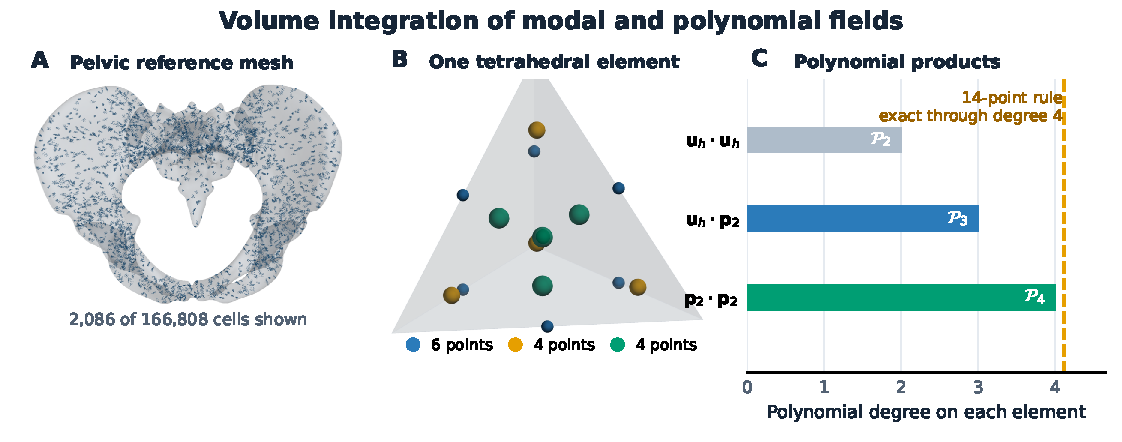
\includegraphics[width=\textwidth,height=0.38\textheight,keepaspectratio]{quadrature_method.pdf}
\caption{\textbf{Volume quadrature for the whole-pelvis displacement decomposition.}
\textbf{(A)} Reference pelvic mesh with actual quadrature positions displayed for every 80th tetrahedron, solely to make the volume sampling visible; the computation uses all $166\,808$ cells.
\textbf{(B)} The positive 14-point degree-4 Basix rule in one reference tetrahedron. Colour and sphere size distinguish its three weight groups (six, four, and four points); weights are positive and sum to the tetrahedral volume.
\textbf{(C)} Polynomial degrees of the squared $P_1$ FE displacement, its cross-product with a quadratic dictionary field, and the quadratic dictionary Gram product. The 14-point rule is exact through degree 4 on each tetrahedron. The illustrations show sampling geometry, not subject-specific deformation.}
\label{fig:quadrature-method}
\end{figure}

\subsubsection{Infinitesimal rigid-body motion elimination}
Infinitesimal rigid-body displacements in $\mathbb{R}^3$ constitute a 6-dimensional linear Lie algebra subspace $\mathfrak{se}(3)$ consisting of 3 translations and 3 rotations:
\begin{equation}
\begin{gathered}
\mathbf u_{\rm rigid}(\mathbf x) = \mathbf t + \boldsymbol\omega \times (\mathbf x - \mathbf x_c), \\
 \mathbf t, \boldsymbol\omega \in \mathbb{R}^3,
\label{eq:rigid-field}
\end{gathered}
\end{equation}
where $\mathbf x_c$ is the volume-weighted spatial centroid of the pelvic domain,
\begin{equation}
\mathbf x_c = \langle \mathbf x \rangle_V = \sum_{p=1}^{N_q} \tilde w_p \, \mathbf x_p.
\end{equation}
To ensure scale-free, dimensionally consistent kinematics across subjects, we define the reference gyration radius $r_g$ and non-dimensionalised anatomical coordinates $\tilde{\mathbf x} = (\tilde x, \tilde y, \tilde z)^\top$:
\begin{equation}
\begin{gathered}
r_g = \sqrt{\langle \|\mathbf x - \mathbf x_c\|^2 \rangle_V} = \sqrt{\sum_{p=1}^{N_q} \tilde w_p \|\mathbf x_p - \mathbf x_c\|^2}, \\
\tilde{\mathbf x} = \frac{\mathbf x - \mathbf x_c}{r_g}.
\label{eq:dimless-coords}
\end{gathered}
\end{equation}
Here the Cartesian coordinate directions correspond to the standard anatomical axes: $x$ is mediolateral (ML), $y$ is anteroposterior (AP), and $z$ is craniocaudal (CC).

In the discrete quadrature representation, each displacement field is a stacked vector $\mathbf U \in \mathbb{R}^{3N_q}$ with components $U_{3p-3+i} = \sqrt{\tilde w_p} \, u_i(\mathbf x_p)$ for $i \in \{1,2,3\}$.
The 6 rigid-body design modes $\mathbf r_1, \dots, \mathbf r_6 \in \mathbb{R}^{3N_q}$ (corresponding to unit translations along $x,y,z$ and unit infinitesimal rotations about $x,y,z$) form the rigid design matrix $\mathbf R \in \mathbb{R}^{3N_q \times 6}$.
We compute its thin QR decomposition,
\begin{equation}
\begin{gathered}
\mathbf R = \mathbf Q_{\rm rigid} \mathbf R_{\rm upper}, \\
 \mathbf Q_{\rm rigid} \in \mathbb{R}^{3N_q \times 6}, \quad \mathbf Q_{\rm rigid}^\top \mathbf Q_{\rm rigid} = \mathbf I_6.
\end{gathered}
\end{equation}
The orthogonal projection operator onto the nonrigid displacement subspace is then:
\begin{equation}
\mathbf P_{\rm nonrigid} = \mathbf I_{3N_q} - \mathbf Q_{\rm rigid} \mathbf Q_{\rm rigid}^\top.
\label{eq:nonrigid-proj}
\end{equation}
For any raw modal displacement field $\mathbf u$, the nonrigid component is $\mathbf u_{\rm nonrigid} = \mathbf P_{\rm nonrigid} \mathbf u$, and the total squared displacement norm partitions orthogonally:
\begin{equation}
\begin{gathered}
\|\mathbf u\|_V^2 = \|\mathbf u_{\rm rigid}\|_V^2 + \|\mathbf u_{\rm nonrigid}\|_V^2, \\
f_{\rm nonrigid} = \frac{\|\mathbf u_{\rm nonrigid}\|_V^2}{\|\mathbf u\|_V^2}.
\end{gathered}
\end{equation}
Crucially, rigid rotation is eliminated at this foundational stage: it is neither retained in the target deformation field nor reported as an explained deformation category.
If a displacement field satisfies $\|\mathbf u_{\rm nonrigid}\|_V^2 / \|\mathbf u\|_V^2 \le 10^{-20}$, it is identified as a pure rigid motion and excluded from nonrigid decomposition.

\subsubsection{Canonical 3D polynomial dictionary}
The vector space of polynomial displacement fields $\mathbf u(\tilde{\mathbf x})$ of degree at most 2 in three dimensions has complete algebraic dimension $3 \times \binom{3+2}{2} = \TotalPolyDOFs$.
Subtracting the \RigidDOFs\ degrees of freedom of infinitesimal rigid motion leaves an exact \NonrigidDOFs-dimensional nonrigid polynomial quotient space.
We decompose this space into four canonical physical deformation families spanning all \NonrigidDOFs\ nonrigid degrees of freedom:
\begin{enumerate}[label=(\roman*)]
\item \textbf{Axial family ($d_{\rm axial} = 6$ degrees of freedom):}
Uniform normal extension/compression along each anatomical axis, together with quadratic normal strain gradients:
\begin{equation}
\begin{aligned}
\mathbf a_{x,1} &= (\tilde x, 0, 0)^\top, \\
 \mathbf a_{x,2} &= (\tfrac{1}{2}\tilde x^2, 0, 0)^\top, \\
\mathbf a_{y,1} &= (0, \tilde y, 0)^\top, \\
 \mathbf a_{y,2} &= (0, \tfrac{1}{2}\tilde y^2, 0)^\top, \\
\mathbf a_{z,1} &= (0, 0, \tilde z)^\top, \\
 \mathbf a_{z,2} &= (0, 0, \tfrac{1}{2}\tilde z^2)^\top.
\end{aligned}
\label{eq:axial-family}
\end{equation}

\item \textbf{Bending family ($d_{\rm bending} = 6$ degrees of freedom):}
Classical pure Euler-Bernoulli flexural modes.
For any pair of distinct coordinate axes $i \ne j \in \{x, y, z\}$, the displacement field
\begin{equation}
\mathbf b_{ij} = \tfrac{1}{2}\tilde x_i^2 \mathbf e_j - \tilde x_i \tilde x_j \mathbf e_i
\label{eq:bending-family}
\end{equation}
satisfies $\partial_i u_j = \tilde x_i$ and $\partial_j u_i = -\tilde x_i$.
Consequently, the Cauchy shear strain vanishes identically:
\begin{equation}
\varepsilon_{ij}(\mathbf b_{ij}) = \tfrac{1}{2}\big(\partial_j u_i + \partial_i u_j\big) = \tfrac{1}{2}\big(-\tilde x_i + \tilde x_i\big) \equiv 0.
\end{equation}
The six ordered pairs $(x,y)$, $(x,z)$, $(y,x)$, $(y,z)$, $(z,x)$, $(z,y)$ thus define six independent shear-free flexural modes.

\item \textbf{Shear family ($d_{\rm shear} = 10$ degrees of freedom):}
Comprises three uniform transverse shears, six planar quadratic transverse shear gradients, and one triaxial cross-gradient shear field $\mathbf w$:
\begin{equation}
\begin{aligned}
\mathbf s_{xy,1} &= (\tilde y, \tilde x, 0)^\top, \\
 \mathbf s_{xy,2} &= (\tilde x \tilde y, \tfrac{1}{2}\tilde x^2, 0)^\top, \\
 \mathbf s_{yx,2} &= (\tfrac{1}{2}\tilde y^2, \tilde y \tilde x, 0)^\top, \\
\mathbf s_{yz,1} &= (0, \tilde z, \tilde y)^\top, \\
 \mathbf s_{yz,2} &= (0, \tilde y \tilde z, \tfrac{1}{2}\tilde y^2)^\top, \\
 \mathbf s_{zy,2} &= (0, \tfrac{1}{2}\tilde z^2, \tilde z \tilde y)^\top, \\
\mathbf s_{zx,1} &= (\tilde z, 0, \tilde x)^\top, \\
 \mathbf s_{zx,2} &= (\tfrac{1}{2}\tilde z^2, 0, \tilde z \tilde x)^\top, \\
 \mathbf s_{xz,2} &= (\tilde x \tilde z, 0, \tfrac{1}{2}\tilde x^2)^\top, \\
\mathbf w &= (\tilde y \tilde z, \tilde x \tilde z, \tilde x \tilde y)^\top = \nabla(\tilde x \tilde y \tilde z).
\end{aligned}
\label{eq:shear-family}
\end{equation}
Unlike bending, these modes produce non-zero shear strains $\varepsilon_{ij} \ne 0$.
The triaxial mode $\mathbf w$ is irrotational ($\nabla \times \mathbf w = \mathbf 0$) and divergence-free ($\nabla \cdot \mathbf w = 0$), completing the chosen basis of the \NonrigidDOFs-dimensional nonrigid polynomial quotient; the complement is not unique.

\item \textbf{Torsion family ($d_{\rm torsion} = 2$ degrees of freedom):}
Saint-Venant torsional twist gradients around the three Cartesian axes:
\begin{equation}
\mathbf t_x = (0, -\tilde x \tilde z, \tilde x \tilde y)^\top, \quad
\mathbf t_y = (\tilde y \tilde z, 0, -\tilde x \tilde y)^\top, \quad
\mathbf t_z = (-\tilde y \tilde z, \tilde x \tilde z, 0)^\top.
\label{eq:torsion-family}
\end{equation}
Each torsion field exhibits identically zero normal strain ($\varepsilon_{xx} = \varepsilon_{yy} = \varepsilon_{zz} \equiv 0$).
Crucially, these three vector fields satisfy the identity:
\begin{equation}
\mathbf t_x + \mathbf t_y + \mathbf t_z \equiv \mathbf 0.
\end{equation}
Hence, this selected torsion-like polynomial family has algebraic dimension 2, spanned by $\{\mathbf t_x, \mathbf t_y\}$.
\end{enumerate}

Figure~\ref{fig:dictionary-families} shows one representative field from each family on the same reference anatomy. The visualisations display the polynomial fields after the rigid-motion projection used in the decomposition; they do not depict separate eigenmodes or unique physical mechanisms.

\begin{figure}[!t]
\centering
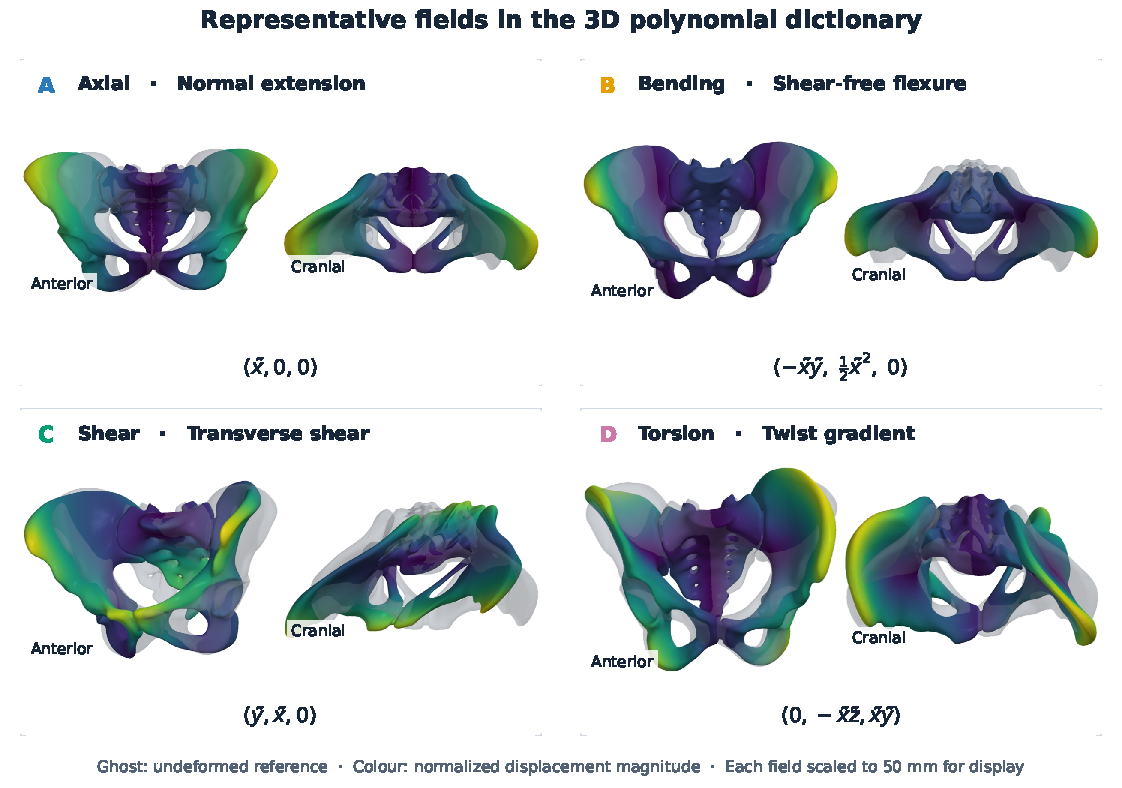
\includegraphics[width=\textwidth,height=0.64\textheight,keepaspectratio]{deformation_families.pdf}
\caption{\textbf{Representative fields of the 3D polynomial deformation dictionary.}
One example per family is evaluated on the reference pelvis: \textbf{(A)} axial extension, $\mathbf a_{x,1}$; \textbf{(B)} shear-free bending, $\mathbf b_{xy}$; \textbf{(C)} uniform transverse shear, $\mathbf s_{xy,1}$; and \textbf{(D)} torsion-like twist, $\mathbf t_x$.
Each card shows anterior and cranial views. Grey denotes the undeformed geometry; colour indicates displacement magnitude relative to the maximum within that field. The formulas are the raw polynomial dictionary members in dimensionless coordinates, and the rendered fields have their volume-weighted infinitesimal rigid component removed. Each rendered field is independently scaled to 50 mm maximum displacement for visibility; these are illustrative basis fields, not computed FE eigenmodes or predicted load responses.}
\label{fig:dictionary-families}
\end{figure}

To assemble the discrete kinematic design matrix, the basis fields in each family $m \in \{\text{axial, bending, shear, torsion}\}$ are sampled at the $N_q$ quadrature points, weighted by $\sqrt{\tilde w_p}$, projected orthogonal to $\mathbf Q_{\rm rigid}$ via $\mathbf P_{\rm nonrigid}$, and orthonormalised via reduced singular value decomposition (SVD):
\begin{equation}
\begin{gathered}
\mathbf P_{\rm nonrigid} \mathbf A_m = \mathbf Q_m \mathbf \Sigma_m \mathbf V_m^\top, \\
 \mathbf Q_m \in \mathbb{R}^{3N_q \times d_m}, \quad \mathbf Q_m^\top \mathbf Q_m = \mathbf I_{d_m}.
\end{gathered}
\end{equation}
The concatenated design matrix $\mathbf A = [\mathbf Q_{\rm axial}, \mathbf Q_{\rm bending}, \mathbf Q_{\rm shear}, \mathbf Q_{\rm torsion}] \in \mathbb{R}^{3N_q \times \NonrigidDOFs}$ spans the complete \NonrigidDOFs-dimensional canonical nonrigid deformation subspace.

\subsubsection{Numerical conditioning, family non-orthogonality, and the Gram matrix}
It is important to note that the four canonical deformation families exhibit intrinsic non-orthogonality and are not mutually orthogonal even on an idealized symmetric domain.
For example, on the symmetric unit cube $[-1, 1]^3$ (volume $V = 8$), the unnormalized continuum volume integral between the bending mode $\mathbf b = (-xy, \frac{1}{2}x^2, 0)^\top$ and the shear mode $\mathbf s = (xy, \frac{1}{2}x^2, 0)^\top$ evaluates analytically to $\int_{[-1, 1]^3} \mathbf b \cdot \mathbf s \, \mathrm dV = -22/45 \approx -0.4889$, corresponding to a volume-normalized inner product $\langle \mathbf b, \mathbf s \rangle_V = \frac{1}{V}\int_{[-1, 1]^3} \mathbf b \cdot \mathbf s \, \mathrm dV = -11/180 \approx -0.0611$ (angular cosine $\cos\theta = -11/29 \approx -0.3793$).
Both example fields have the same nonzero mean translation $(0,1/6,0)^\top$. After subtracting it, their volume-normalised inner product is $-4/45$ and their cosine is $-2/3$. Thus non-orthogonality also holds after the rigid-motion projection used here. This does not mean the two families have a nonzero vector in their intersection.

On the real, geometrically asymmetric pelvic ring, this intrinsic non-orthogonality combines with anatomical geometry.
The kinematic design matrix $\mathbf A$ has 2-norm condition number $\kappa(\mathbf A) \approx \DesignConditionNumber$, and the associated Gram matrix $\mathbf G = \mathbf A^\top \mathbf A \in \mathbb{R}^{\NonrigidDOFs \times \NonrigidDOFs}$ has condition number:
\begin{equation}
\kappa(\mathbf G) = \frac{\sigma_{\max}(\mathbf G)}{\sigma_{\min}(\mathbf G)} = \kappa(\mathbf A)^2 \approx \GramConditionNumber.
\end{equation}
A Gram condition number of $\sim21$ indicates that the sampled design columns were linearly independent to numerical precision at the reported geometry; it does not establish unique physical attribution to the families.

\subsubsection{Cooperative game-theoretic Shapley value norm allocation}
Because the four deformation subspaces exhibit intrinsic non-orthogonality (shared explained norm) and cannot be mutually orthogonal, projecting onto them sequentially (e.g., Gram-Schmidt orthogonalisation) would introduce an arbitrary, order-dependent bias: the first chosen family would absorb all shared variance, artificially starving subsequent families.
To obtain an order-independent allocation conditional on this chosen dictionary, we formulate the problem using cooperative game theory.

Let $M = \{\text{axial}, \text{bending}, \text{shear}, \text{torsion}\}$ denote the set of four pattern players ($|M| = 4$).
There are $2^4 = 16$ possible coalitions $S \subseteq M$.
For any coalition $S$, we construct the concatenated family design matrix $\mathbf A_S \in \mathbb{R}^{3N_q \times \sum_{m \in S} d_m}$ and define the characteristic function $v(S)$ as the fraction of nonrigid squared displacement norm explained by the joint subspace:
\begin{equation}
\begin{gathered}
v(S) = R^2(S) = \frac{\mathbf u_{\rm nonrigid}^\top \mathbf P_S \mathbf u_{\rm nonrigid}}{\|\mathbf u_{\rm nonrigid}\|_V^2}, \\
\mathbf P_S = \mathbf A_S (\mathbf A_S^\top \mathbf A_S)^+ \mathbf A_S^\top,
\label{eq:coalition-r2}
\end{gathered}
\end{equation}
with $v(\emptyset) = 0$, where $(\cdot)^+$ denotes the Moore-Penrose pseudoinverse.
The Shapley value $f_m$ is uniquely specified by the following axioms for this chosen coalition value function and set of families:
\begin{enumerate}
\item \textbf{Efficiency:} The sum of allocated values equals the value of the grand coalition:
\begin{equation}
\sum_{m \in M} f_m = v(M) = R^2(M) = 1 - f_{\rm residual}.
\end{equation}
\item \textbf{Symmetry:} If two families $m, k \in M$ contribute identically to every coalition ($v(S \cup \{m\}) = v(S \cup \{k\})$ for all $S \subseteq M \setminus \{m, k\}$), then $f_m = f_k$.
\item \textbf{Dummy player:} If a family $m$ adds zero marginal variance to every coalition ($v(S \cup \{m\}) = v(S)$ for all $S \subseteq M \setminus \{m\}$), then $f_m = 0$.
\item \textbf{Additivity:} For any two characteristic value functions $v$ and $w$ defined on the same set of players, the values allocated under the combined sum game $(v + w)(S) = v(S) + w(S)$ satisfy $\phi_m(v + w) = \phi_m(v) + \phi_m(w)$.
\end{enumerate}
The explicit Shapley allocation formula evaluates the marginal contribution of family $m$ averaged over all coalition orders:
\begin{equation}
f_m = \sum_{S \subseteq M \setminus \{m\}} \frac{|S|!(|M| - |S| - 1)!}{|M|!} \Big[ v\big(S \cup \{m\}\big) - v(S) \Big].
\label{eq:shapley-formula}
\end{equation}
The unexplained shape change is retained as an explicit residual:
\begin{equation}
f_{\rm residual} = 1 - v(M) = 1 - R^2(\text{axial} \cup \text{bending} \cup \text{shear} \cup \text{torsion}).
\end{equation}
Because subspace projection operators are monotonic ($V_S \subseteq V_{S \cup \{m\}} \implies v(S \cup \{m\}) \ge v(S)$), every marginal contribution is non-negative, which guarantees $f_m \ge 0$ for all $m$.
Exact closure holds identically:
\begin{equation}
f_{\rm axial} + f_{\rm bending} + f_{\rm shear} + f_{\rm torsion} + f_{\rm residual} \equiv 1.0000 \quad (100.0\%).
\end{equation}
Furthermore, the fractions are strictly scale-invariant ($\mathbf u \mapsto c\mathbf u$ for $c \ne 0$) and sign-invariant ($\mathbf u \mapsto -\mathbf u$).
For comparative diagnostics, we also compute the standalone coefficient of determination for each isolated family:
\begin{equation}
R^2_m = v(\{m\}) = \frac{\mathbf u_{\rm nonrigid}^\top \mathbf P_m \mathbf u_{\rm nonrigid}}{\|\mathbf u_{\rm nonrigid}\|_V^2}.
\end{equation}
Due to the intrinsic geometric coupling between families ($\kappa(\mathbf G) \approx \GramConditionNumber$), the sum $\sum_{m \in M} R^2_m$ may moderately exceed the total explained fraction $R^2(M)$; the Shapley values allocate this overlap in an order-independent way conditional on the selected dictionary and anatomical axes.

\subsection{Load routing and modal strain-energy fractions}
\label{sec:routing-methods}

For each load case we solved the static problem $K_s\mathbf u_s=\mathbf b$ on $\Omega_{\rm ref}$, projected the result onto the $M_s$-orthonormal eigenbasis $\Phi$,
\begin{equation}
q=\Phi^\top M_s\mathbf u_s,\qquad E_i=\tfrac12\lambda_i q_i^2,\qquad f_i=\frac{E_i}{\sum_{j=1}^{N_{\rm ev}} E_j},
\label{eq:modal-fraction}
\end{equation}
and summarised each pathway's contribution by its retained modal strain-energy fraction $f_i$ evaluated across the $N_{\rm ev}=15$ computed modes.
Block throughput for a clustered regime $C$ is $f_C=\sum_{i\in C}f_i$, and the dominant mode set $N_{80}$ of a load case is the smallest subset of modes (selected in descending order of mean energy contribution) whose cumulative mean energy fractions reach at least 0.80.
For cross-load comparison we also report cosine similarity of full 15-mode mean profiles and Jaccard overlap of dominant mode sets.


\subsection{First-order eigenvalue sensitivities and analytical uncertainty propagation}
\label{sec:sensitivities}

To propagate material-parameter uncertainty to the spectrum without repeated finite-element solves, we use classical first-order sensitivities of the generalised eigenproblem~\eqref{eq:gep}: for a parameter $p_j$ that affects only the stiffness,
\begin{equation}
\frac{\partial\lambda_m}{\partial p_j}
=\frac{\boldsymbol\phi_m^\top\,(\partial K_s/\partial p_j)\,\boldsymbol\phi_m}
{\boldsymbol\phi_m^\top M_s\,\boldsymbol\phi_m}.
\label{eq:ev-sensitivity}
\end{equation}
For ligament parameters, derivatives of local $3\times3$ blocks are $\partial W/\partial k_{\rm seg}=\mathbf e\mathbf e^\top$ and $\partial W_g/\partial T_{\rm seg}=(I-\mathbf e\mathbf e^\top)/L$. They enter the signed $6\times6$ segment assembly, with factor $1/N_{\rm seg}$ for differentiation with respect to a bundle parameter.
For cartilage moduli, $\partial K_s/\partial E_{\rm region}$ is the element-wise elastic stiffness integrated over the corresponding joint domain, scaled by the baseline modulus.
At source points on the high-density branch of~\eqref{eq:keller}, $\partial E/\partial\alpha=\rho_{\rm ash}^{\beta}$ and $\partial E/\partial\beta=\alpha\rho_{\rm ash}^{\beta}\ln\rho_{\rm ash}$; the derivatives vanish on the constant branch. We interpolate each source derivative with the same radial-basis-function operator used for the modulus, then integrate it against the modal strain-energy density. This differentiates the implemented map, in which the nonlinear density law precedes interpolation. A finite-difference check at 1669 sampled cells in one subject agreed to relative $L^2$ errors below $4\times10^{-11}$ for both parameters.
Storing the dimensionless Jacobians
\begin{equation}
J_j^{(m)}=\frac{p_j}{\lambda_m}\frac{\partial\lambda_m}{\partial p_j}
\end{equation}
once per subject lets us compute first-order log-space variance propagation as $\mathrm{Var}(\log\lambda_m) \approx \mathbf J_m^\top \Sigma_{\log p} \mathbf J_m$ for an assumed covariance $\Sigma_{\log p}=\mathrm{Cov}(\log\mathbf p)$ on the material parameters. The implemented scenarios use log-space standard deviations $(0.25,0.20,0.10)$ for global, type, and side effects of ligament stiffness; $(0.35,0.25,0.12)$ for ligament pretension; and $(0.35,0.25,0.10)$ for cartilage modulus. The global ligament stiffness--pretension correlation is 0.50. Bone-law parameters $\alpha$ and $\beta$ have log-space standard deviations 0.30 and 0.20 with correlation $-0.40$. These are assumed scenarios, not parameters estimated from the cohort. Eigenvalue CoVs use the lognormal conversion $\sqrt{\exp(v)-1}$ from propagated log-variance $v$.
For adjacent eigenvalues $\lambda_i, \lambda_{i+1}$, the variance of the gap $\Delta\lambda = \lambda_{i+1}-\lambda_i$ is computed from the combined sensitivity vector $\mathbf g_{i,i+1} = \lambda_{i+1}\mathbf J_{i+1} - \lambda_i\mathbf J_i$ as
\begin{equation}
\mathrm{Var}(\lambda_{i+1}-\lambda_i) \approx \mathbf g_{i,i+1}^\top \Sigma_{\log p}\,\mathbf g_{i,i+1} \approx \mathrm{Var}(\lambda_{i+1}) + \mathrm{Var}(\lambda_i) - 2\,\mathrm{Cov}(\lambda_i, \lambda_{i+1}),
\label{eq:gap-cov}
\end{equation}
accounting for the substantial positive covariance induced by shared tissue parameters.
The gap signal-to-noise ratio compares the nominal gap with its propagated standard deviation (Section~\ref{sec:uq-results}). It measures local susceptibility of modal ordering under the specified parameter covariance. These gap diagnostics do not directly propagate uncertainty in eigenvectors or anatomical capacities and therefore do not establish subspace robustness under large parameter changes. Sex-stratified summaries and combined uncertainty results are reported in Sections~\ref{sec:details-B} and~\ref{sec:details-D}.

\subsection{Decomposition of variability sources and robustness analyses}
\label{sec:robustness-methods}

To separate shape and material contributions to spectral variability, we compared the full cohort against a shape-only cohort ($\chi_s$, fixed reference bone modulus) and a material-only cohort (identity deformation, subject-specific bone modulus).
Robustness was assessed by (i)~random permutation of subject order, (ii)~a 500-replicate bootstrap of 222 draws with replacement at the fixed threshold and a separate 2,000-replicate bootstrap of 278 draws with replacement and threshold re-estimation, and (iii)~morphology-axis permutation null tests in which a one-dimensional anatomical proxy $\mu$ (e.g.\ AP inlet diameter) was shuffled 1000 times to assess whether swap-rate localisation along $\mu$ exceeded chance (Table~\ref{tab:detail-A6}).
Post-hoc allometric regressions of $\log\lambda_k$ on isotropic body-size scale~$s$ (with instrumental variables from volume, surface, and mass) and Shapley/LMG variance decomposition into scale, sex, shape, and material contributions are reported in Section~\ref{sec:details-D}.

\subsection{Minimal analytical model for the near-degenerate regime}
\label{sec:toy-methods}

The cluster/subspace framework admits a compact analytical interpretation via a two-degree-of-freedom model.
Let $q_1,q_2$ denote two generalised rotational coordinates and define a stiffness matrix
\begin{equation}
K_2=\begin{bmatrix} k_1 & c\\ c & k_2\end{bmatrix},\qquad \Delta=k_1-k_2,\qquad k_1,k_2>0,\ k_1k_2>c^2,
\end{equation}
with detuning~$\Delta$ and coupling~$c$.
The eigenvalues are
\begin{equation}
\lambda_{\pm}=\frac{k_1+k_2}{2}\pm\sqrt{\Big(\tfrac{\Delta}{2}\Big)^2+c^2},
\qquad
\tan(2\theta)=\frac{2c}{\Delta},
\label{eq:2dof-eig}
\end{equation}
and the minimum separation $\lambda_+-\lambda_-=2|c|$ is attained at $\Delta=0$, for constant nonzero $c$ as $\Delta$ is varied. With a continuous branch convention, $2\theta=\operatorname{atan2}(2c,\Delta)$; at $\Delta=0$ the angle is $\pi/4$ for $c>0$, up to eigenvector sign. When $c=0$, an exact crossing occurs.
The operational criterion
\begin{equation}
|\Delta(\mu)|\le\tau\,|c(\mu)|\quad\text{for some morphology parameter }\mu,\qquad \tau\in[1.5,2],
\label{eq:2dof-criterion}
\end{equation}
separates near-degenerate/mixing from stable-ordering regimes.
Adding a third coordinate $q_3$ with stiffness~$s$ and coupling vector $\mathbf d = [d_1, d_2]^\top$, dynamic reduction of the $3\times 3$ eigenproblem $(K - \lambda I)\mathbf q = \mathbf 0$ gives the exact non-linear reduced eigenproblem
\begin{equation}
\Big( K_2 - \frac{\mathbf d \mathbf d^\top}{s - \lambda} \Big) \mathbf q_{12} = \lambda \mathbf q_{12}.
\label{eq:dynamic-schur}
\end{equation}
In the low-frequency limit ($\lambda \ll s$), static condensation yields the linear effective stiffness
\begin{equation}
K_{\rm eff} = K_2 - \frac{\mathbf d \mathbf d^\top}{s} = \begin{bmatrix} k_1-d_1^2/s & c-d_1d_2/s\\ c-d_1d_2/s & k_2-d_2^2/s\end{bmatrix},
\label{eq:schur}
\end{equation}
showing how coupling to an additional coordinate shifts effective detuning and coupling. Depending on the parameters, the shift can move the system toward or away from avoided crossing. The assumption $\lambda\ll s$ excludes using this condensation for an arbitrarily soft hidden coordinate.
In all stochastic numerical simulations (Section~\ref{sec:toy-results}), the full $3\times 3$ eigenproblem is solved directly without static or dynamic truncation.
In the $n$-DOF finite-element setting, the detected clusters correspond to $\{q_1,q_2\}$, the canonical basis $(\boldsymbol\psi_1,\boldsymbol\psi_2)$ to the rotated eigenvectors, and $\mathrm{gap}_{\rm in}$ to $(\lambda_+-\lambda_-)/\lambda_-$.
A stochastic population instantiation of this model, evaluated in Section~\ref{sec:toy-results}, reproduces the label--subspace dissociation, the standing-vs-task routing contrast, and the effect of hidden-pathway variability observed in the full pelvic cohort.
The stochastic model used in the figure is specified in Section~\ref{sec:toy-specification}. Static condensation is only a limiting argument; it is not used for the reported stochastic eigensolves.

\subsubsection{Stochastic implementation}\label{sec:toy-specification}
This specification defines the stochastic implementation evaluated in Section~\ref{sec:toy-results}. Parameters are dimensionless and illustrative; they were not fitted to the pelvic cohort. The stiffness matrix is
\begin{equation}
K=\begin{bmatrix}12+\Delta/2&c&d_1\\c&12-\Delta/2&d_2\\d_1&d_2&s\end{bmatrix},\qquad M=I.
\end{equation}
For morphology coordinate $\mu$ and nuisance scale $\eta$, independent standard-normal draws determine
\begin{align}
\Delta&=1.6\mu+(0.05+0.22\eta)Z_\Delta,\\
c&=|0.22+(0.008+0.018\eta)Z_c|,\\
s&=5.2\exp[(0.02+0.12\eta)Z_s],\\
d_1&=0.28+0.42\eta+(0.01+0.08\eta)Z_1,\\
d_2&=0.24+0.40\eta+(0.01+0.08\eta)Z_2.
\end{align}
Draws are accepted only when all eigenvalues exceed $10^{-10}$ and the largest absolute component of the third coordinate occurs in the lowest eigenvector. The low-rank backbone is therefore conditioned by construction, not independently discovered in this example. Up to 200 draws are attempted per subject.

The anatomical observable and task-like load are the unit-normalised vector $(1,0,0.2)^\top$; the standing-like load is the unit-normalised vector $(0.10,0.05,1)^\top$. For unit-normalised eigenvectors $\mathbf v_i$, the observable projection is $(\mathbf v_i^\top\mathbf b)^2$ and the upper-pair score is the sum for $i=2,3$. Load fractions are proportional to $(\mathbf v_i^\top\mathbf f)^2/\lambda_i$. These squared projections differ from the max-nodal anatomical capacity used in the finite-element cohort and serve only as analogous illustrative observables.

The main illustrative cohort contains 240 evenly spaced coordinates in $[-1.10,1.10]$, perturbed by normal noise of standard deviation 0.035 (random seed 11), sorted, and simulated at $\eta=0.85$ (seed 19). The nuisance sweep uses nine values in $[0,1.6]$ and 480 coordinates in $[-0.35,0.35]$, with seed 31 at each value. Carrier change is the proportion whose larger upper-pair observable projection changes rank relative to $\eta=0$. Pair projection and task routing are summarised by their medians.

The full $3\times3$ eigenproblem is solved for every accepted draw. The static-condensation formula in Eq.~\eqref{eq:schur} is a limiting argument valid for $\lambda\ll s$; it is not an approximation used for the upper-pair eigenvalues in this example. The model illustrates rank redistribution under specified parameter variation and does not validate a particular pelvic tissue mechanism.


\subsection{Statistical analysis}
\label{sec:statistics}

All statistical analyses were executed using SciPy, statsmodels, and custom Python routines.
Continuous metrics across non-normal cohorts were evaluated using non-parametric methods.
Two-group comparisons (e.g., non-swapped vs.\ swapped cluster members, or male vs.\ female distributions) were conducted using two-sided Mann--Whitney $U$ tests.
Effect sizes for Mann--Whitney tests are reported as rank-biserial correlations $r_{\rm rb}=1-2U_1/(n_1n_2)$, where $U_1$ is computed for the first listed group. With this orientation, positive values indicate larger observations in the second group; the statistic equals Cliff\textquotesingle s delta for second versus first group.
Paired differences across loading conditions or mode pairs were assessed via two-sided Wilcoxon signed-rank tests.
Bivariate associations between continuous anatomical dimensions (such as AP inlet diameter or isotropic scale) and modal metrics (energy fractions, spectral gaps) were quantified using Spearman's rank correlation coefficient $\rho_s$.
The four pre-specified rank-versus-capacity comparisons in each label-exchange table were adjusted with the Benjamini--Hochberg procedure. Other exploratory test families were not uniformly adjusted; their raw $p$-values should not be treated as confirmatory discoveries.
Confidence intervals for median differences and median ratios in the label-exchange comparisons were obtained by percentile bootstrap resampling (5,000 independent within-group resamples; random seed 20260918), using the 2.5th and 97.5th percentiles. Mann--Whitney probabilities concern distributional differences and should not be interpreted as tests specifically of the median difference.
Cohort-level cluster stability was evaluated by repeating the detection pipeline across 500 random subcohort draws of 80\% sample size performed with replacement ($m = 222$), yielding 95\% bootstrap stability intervals.
Separate prevalence intervals used 2,000 replicates of 278 draws with replacement and threshold re-estimation (seed 20260918). These are resampling summaries, not independent biological validation.

Differences in subspace orientation across the cohort were quantified using the Grassmann distance $d_G(Q_{\rm ref}, Q_s) = \|\boldsymbol\theta\|_2$.
Importantly, $d_G$ measures the intrinsic geometric distance between the linear subspaces $\mathrm{span}(Q_{\rm ref})$ and $\mathrm{span}(Q_s)$ in the Grassmannian manifold $\mathrm{Gr}(r, n)$, which is strictly invariant to arbitrary unitary rotations of the internal basis within either subspace.
Variation in $d_G$ cannot be caused by internal basis re-indexing, although sex-group differences in distance to one reference do not by themselves establish a direction of subspace shift or rule out reference effects.

\subsection{Software and computational implementation}


Finite-element assembly, eigensolves, and postprocessing were implemented in Python~3.11 with DOLFINx/FEniCSx~($\ge$0.10), PETSc, and SLEPc.
Reported figures, tables, and numerical values were produced by the study analysis scripts; a public code archive has not yet been established.
Results are stored as compressed Zarr arrays for reproducible downstream analysis.
The formulation and stochastic implementation are specified above; a public source-code release remains to be prepared.

% ============================================================
An OpenAI language model assisted the restructuring and drafting of this manuscript and cover letter from the existing manuscript and analysis outputs. The revised numerical analyses were executed with the documented project scripts and checked against the archived finite-element fields; the authors retain responsibility for the scientific content.

\section{Results}
\label{sec:results}

\subsection{Reference deformation atlas and numerical validation}\label{sec:details-E}
\label{sec:global-deformation-results}

This analysis provides the reference-mode atlas, synthetic validation checks, and full deformation profiles. The mathematical formulation, 14-point degree-4 quadrature, rigid-motion projection, polynomial dictionary, and Shapley allocation are given in the Methods.
Table~\ref{tab:detail-E1} tabulates the complete 15-mode quantitative profile across all four canonical deformation families, standalone $R^2$ values, and residual fractions.
Table~\ref{tab:detail-E2} reports the synthetic benchmark validations across idealized symmetric and irregular pelvic domains.

\begin{figure}[p]
  \centering
  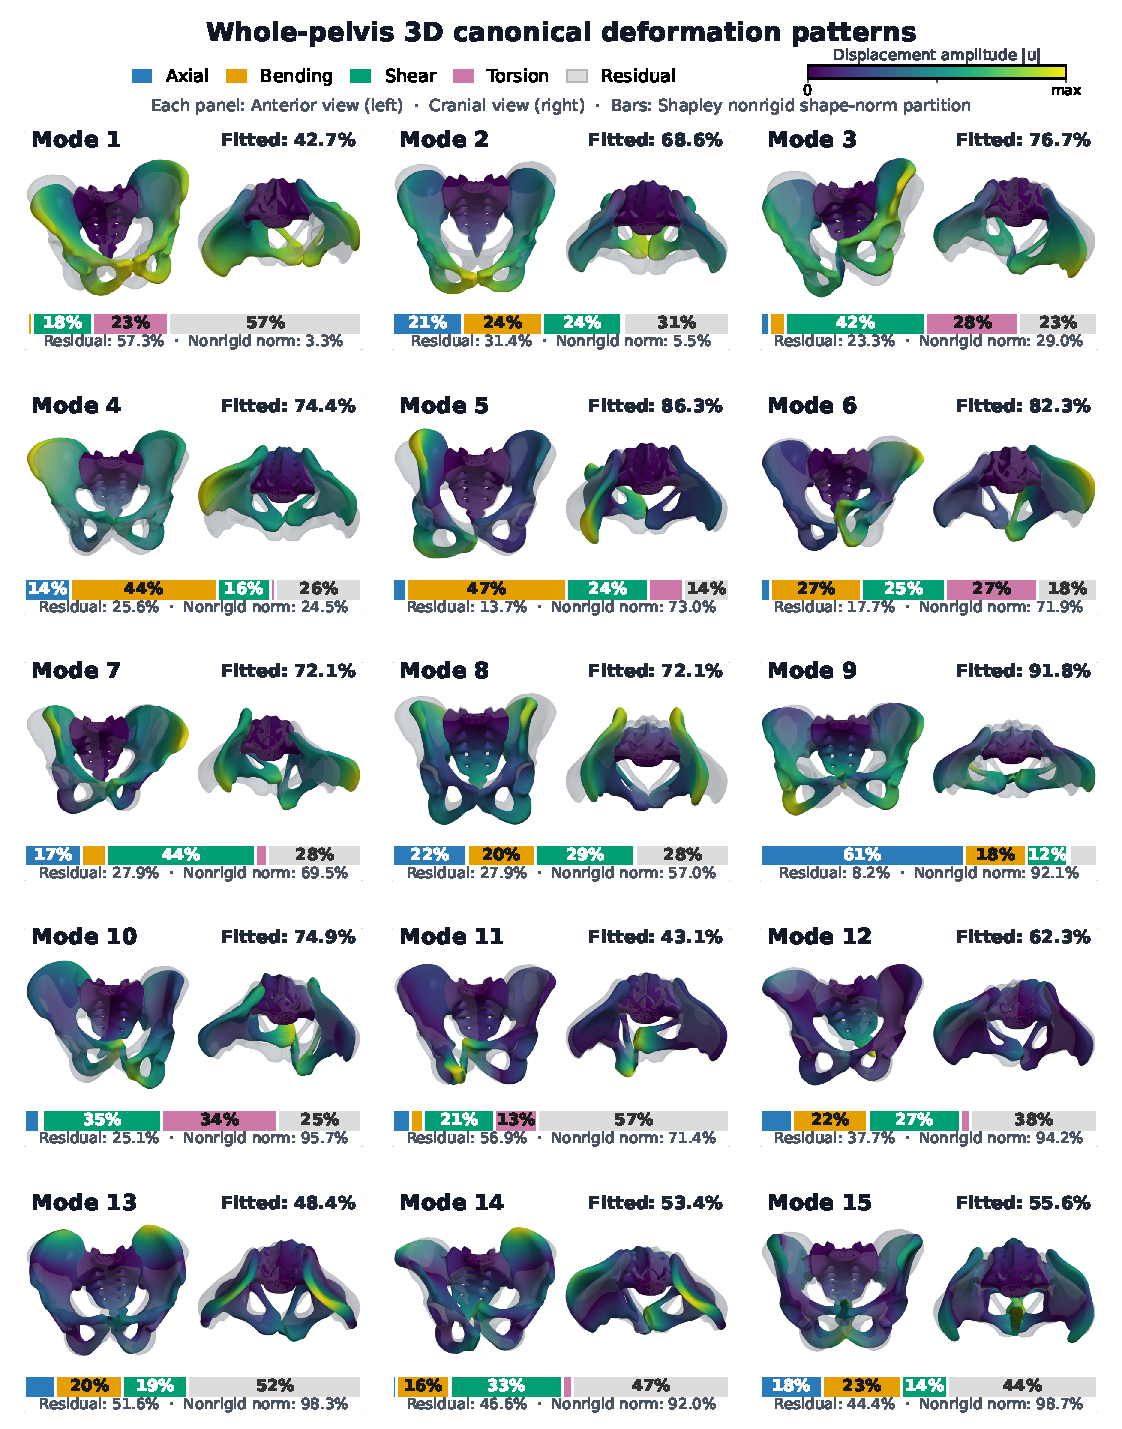
\includegraphics[width=\linewidth,height=0.79\textheight,keepaspectratio]{reference_mode_atlas.pdf}
  \begingroup
  \fontsize{9}{10.5}\selectfont
  \caption{\textbf{Whole-pelvis deformation patterns of reference modes.}
  Anterior (left) and cranial (right) views show displacement magnitude from purple to yellow, scaled to a 50~mm maximum; grey geometry is undeformed.
  Each bar partitions the whole-pelvis nonrigid squared shape norm into fitted axial tension/compression, bending, transverse shear, torsion, and residual.
  Infinitesimal rigid-body translation and rotation are projected out upfront; rigid rotation is not a reported deformation category.
  The decomposition operates in full 3D Cartesian space across the entire pelvic ring without imposing a 1D reference axis.
  Overlapping pattern subspaces are allocated using Shapley values.
  ``Fitted'' reports the percentage of nonrigid shape change explained by the four canonical 3D families.
  All fractions use the complete continuum without bone-wise subdivision and describe kinematic shape change rather than elastic-energy shares.}
  \label{fig:si-atlas}
  \endgroup
\end{figure}

\subsubsection{Synthetic benchmark and backwards-identification validation}
To verify the accuracy, robustness, and backwards-identifiability of the global deformation decomposition, we executed synthetic validation experiments on both an idealized symmetric domain (cube) and the realistic reference pelvis mesh (Table~\ref{tab:detail-E2}).

On the symmetric domain, pure synthetic fields belonging to the axial, shear, and torsion families are identified with $100.0\%$ fidelity, zero cross-talk, and exactly $0.0\%$ residual.
For pure Euler-Bernoulli bending ($\mathbf u = (-xy, \tfrac{1}{2}x^2, 0)$), the displacement field consists of an axial cross-term $-xy$ and a transverse parabolic deflection $\tfrac{1}{2}x^2$.
Because the quadratic shear mode $\mathbf s_{xy,2} = (xy, \tfrac{1}{2}x^2, 0)$ shares the identical transverse parabolic deflection $\tfrac{1}{2}x^2$, the pure flexural field lies in the joint span $V_{\rm bending} \oplus V_{\rm shear}$.
The equal-weight $15\times15\times15$ grid benchmark allocates $77.5\%$ to bending and $22.5\%$ to shear, with residual rounding to zero. These numbers describe the sampled grid and the chosen Shapley game, not a unique physical decomposition of the field.

On the actual reference pelvis mesh, pure canonical polynomial fields are recovered with exactly $0.0\%$ residual ($100.0\%$ fitted fraction):
\begin{itemize}
\item Pure axial stretch ($x\mathbf e_x$): $85.3\%$ axial share, $0.0\%$ residual ($100.0\%$ fitted).
\item Pure triaxial extension ($x\mathbf e_x - \tfrac{1}{2}y\mathbf e_y - \tfrac{1}{2}z\mathbf e_z$): $84.8\%$ axial share, $0.0\%$ residual ($100.0\%$ fitted).
\item Pure Euler-Bernoulli bending: $74.1\%$ bending share, $0.0\%$ residual ($100.0\%$ fitted).
\item Pure transverse shear: $82.8\%$ shear share, $0.0\%$ residual ($100.0\%$ fitted).
\item Pure torsion-like polynomial field: $87.1\%$ torsion share, $0.0\%$ residual ($100.0\%$ fitted).
\end{itemize}
When subjected to pure infinitesimal rigid translations or pure infinitesimal rotations, the nonrigid fraction is detected as $f_{\rm nonrigid} < 10^{-27}$, correctly triggering the rigid-motion filter and showing negligible contamination in these numerical checks.
Finally, adding arbitrary rigid-body translations and rotations to an axial deformation field yields identical Shapley shares ($85.3\%$ axial, $7.2\%$ bending, $7.5\%$ shear, $0.0\%$ torsion, $0.0\%$ residual) to within machine precision ($< 10^{-10}$), demonstrating invariance to addition of infinitesimal rigid displacement fields, rather than invariance to arbitrary rotation of anatomical axes.

\subsubsection{Reference mode deformation profiles and biomechanical interpretation}
Table~\ref{tab:detail-E1} compiles the quantitative whole-pelvis 3D deformation decomposition for all fifteen reference eigenmodes.
The results resolve several key biomechanical features of the pelvic ring:
\begin{itemize}
\item \textbf{Modes~1 and~2 (low-rank backbone):}
For Mode~1, the nonrigid deformation accounts for $3.3\%$ of the total displacement norm (the remainder reflecting whole-pelvis rocking on the sacroiliac/pubic supports).
Its nonrigid shape change is predominantly out-of-plane torsional twist ($22.7\%$) and transverse shear ($17.7\%$), with a total fitted fraction of $42.7\%$ (residual $57.3\%$).
For Mode~2, nonrigid shape change ($5.5\%$ of total norm) is a coupled sagittal ring flexure and shear ($23.6\%$ bending, $23.7\%$ shear, $20.8\%$ axial, $68.6\%$ fitted, residual $31.4\%$).
The selected 3D displacement dictionary explains more than two-thirds of the nonrigid squared displacement norm; the tested one-axis dictionary gave a lower descriptive fit.

\item \textbf{Modes~4 and~5 (dominant flexural pathways):}
Modes~4 and~5 exhibit strong bending dominance, explaining $43.6\%$ and $47.4\%$ of their nonrigid norm respectively (with standalone bending fits $R^2_{\rm bending}$ reaching $47.6\%$ and $62.4\%$, and total explained fractions of $74.4\%$ and $86.3\%$).
These modes capture lateral and anteroposterior flaring of the iliac wings.

\item \textbf{The inlet-related 9--10 pair:}
Mode~9 is the most highly fitted mode in the entire spectrum ($91.8\%$ explained, residual only $8.2\%$).
Its deformation is overwhelmingly axial ($60.6\%$ Shapley share; standalone $R^2_{\rm axial} = 67.7\%$), consistent with Cartesian normal-extension content. Its relation to inlet opening is evaluated separately with the anatomical diameter functional; the polynomial allocation does not measure circumferential strain.
In contrast, its near-degenerate partner Mode~10 ($74.9\%$ fitted) is dominated by shear ($35.2\%$) and torsion ($34.3\%$), with minimal axial contribution ($4.3\%$; standalone $R^2_{\rm torsion} = 30.3\%$, $R^2_{\rm shear} = 32.7\%$, residual $25.1\%$).
These reference-mode descriptions illustrate distinct kinematic patterns within the pair. Their rank-specific interpretation should not be transferred unchanged across subjects with label exchange.
\end{itemize}


\begin{table*}[!htbp]
\caption{Reference mode whole-pelvis 3D deformation decomposition. }
\label{tab:detail-E1}
\centering
\DetailTableInput{global_deformation_modes_table.tex}
\end{table*}



\begin{table*}[!htbp]
\caption{Synthetic benchmark and backwards-identification validation. }
\label{tab:detail-E2}
\centering
\DetailTableInput{global_deformation_synthetic_table.tex}
\end{table*}




\FloatBarrier
\subsection{Population variability separates an order-locked backbone from recurrent clustered regimes}
\label{sec:spectral-results}

The cohort of $N{=}278$ subjects resolves the spectrum into two regimes: an order-locked low-rank backbone and recurrent higher-rank clustered blocks (Fig.~\ref{fig:spectral-dashboard}, Table~\ref{tab:clusters}).
The reference deformation atlas is provided in Fig.~\ref{fig:si-atlas}. Modes~1--3 are rarely reordered across the cohort (swap rate $<0.4\%$), whereas higher ranks contain small consecutive gaps and frequent label exchange.
Using a data-driven cluster threshold $\varepsilon_{\rm in}\approx 0.131$ (25th percentile of pooled relative consecutive gaps; see Methods), we detect nine near-degenerate rank clusters above a 3\% prevalence floor.
The most prevalent cluster is rank modes~9--10 (\PrevalenceNineTen\% of subjects), followed by rank modes~12--15 (\PrevalenceTwelveFifteen\%) and rank modes~5--6 (\PrevalenceFiveSix\%).
No eigenvalue pair met the operational numerical multiplicity criterion ($\mathrm{gap}_{\rm in} \le 10^{-6}$). No obvious spatial symmetry was identified that would enforce repeated eigenvalues, although accidental degeneracy is not mathematically excluded.

Anatomical variability does not destabilise the spectrum uniformly.
Label fragility is concentrated in a small number of compact families, while low-rank order is preserved.
For the dominant 9--10 and 12--15 clusters, median relative internal gaps are small enough that modest perturbations can reverse local ordering.
The 9--10 block has a larger median external separation than internal gap, whereas the 12--15 regime is left-separated but right-truncated by the eigensolve; the 9--10 pair can therefore be assessed as an interior subspace, whereas conclusions about isolation of 12--15 remain limited.
The result identifies spectral regions in which rank-based comparison is more or less reliable under the present model assumptions.

Permutation statistics reinforce this interpretation.
Modes~12 and~13 exhibit the highest swap rates, and mode~15 also shows a sizeable unpaired fraction under strict cross-subject pairing, whereas the backbone is essentially fixed in its ordering.
For cross-subject modal comparison, the consequence is concrete: while one-to-one modal comparison is well-conditioned for the low-rank backbone, higher-rank comparisons must accommodate mode mixing and label exchange through subspace representations.

A variability decomposition into shape-only and material-only datasets (Fig.~\ref{fig:spectral-dashboard}C) shows that the shape-only dataset has the larger coefficient of variation for modes~1--8, whereas bone-density heterogeneity contributes with increasing relative weight in modes~9--15.
Shape changes alter \emph{how} the spatial density heterogeneity enters the stiffness operator: shape dominates lower modal variance while material heterogeneity contributes increasingly at higher ranks.
The shape-only and material-only coefficients of variation are not additive variance shares, nor do they isolate interactions or establish a causal mechanism for cluster formation.

These prevalence estimates are not driven by a few outliers or by the order in which subjects are processed.
The 500 bootstrap draws of 222 subjects with replacement gave 95\% percentile ranges of 48.2--61.7\% for cluster 9--10 and 35.6--48.6\% for cluster 12--15 (Table~\ref{tab:detail-B1}). A separate 2,000-draw full-cohort bootstrap with threshold re-estimation gave 49.6--59.4\% and 36.7--46.0\%, respectively. Random permutation of subject order leaves cluster prevalence and swap statistics unchanged to machine precision.
The central spectral hierarchy is therefore a cohort-level feature rather than a post-processing artefact.
Additional cluster-mapping, swap, and robustness diagnostics are provided in Section~\ref{sec:details-A} and Section~\ref{sec:details-B}.

\begin{figure}[!t]
  \centering
  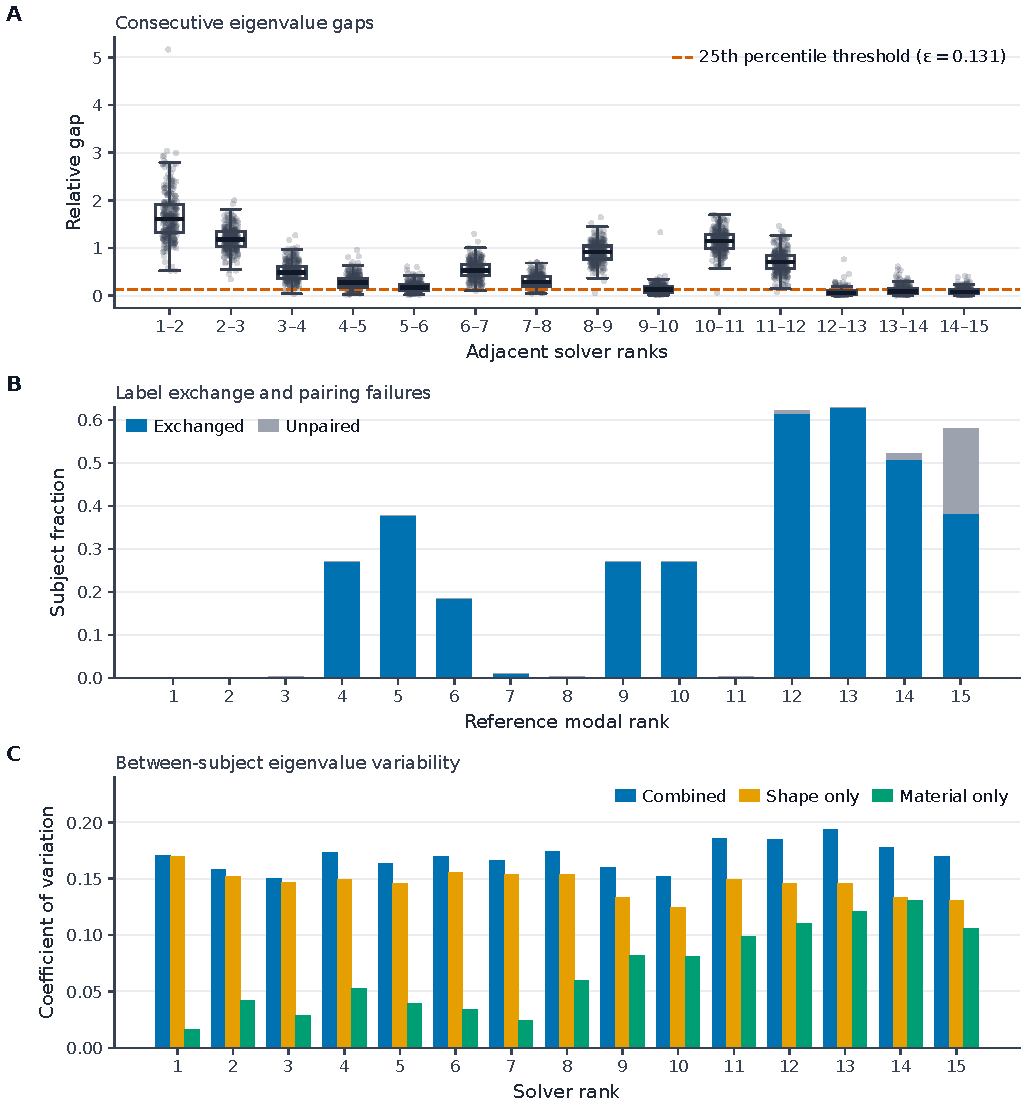
\includegraphics[width=\textwidth]{Fig2.pdf}
  \caption{\textbf{Population variability partitions the stiffness spectrum into an order-locked backbone and clustered higher ranks.}
  \textbf{(A)} Consecutive relative spectral gaps $\mathrm{gap}_{\rm in}(i) = (\lambda_{i+1}-\lambda_i)/\lambda_i$ across the cohort ($N{=}278$); the dashed line marks the data-driven cluster threshold $\varepsilon_{\rm in} \approx 0.131$ (25th percentile).
  \textbf{(B)} Subject fraction exhibiting label exchange (blue) and unpaired pairing failures (grey; $\mathrm{MAC}_{M_0} < 0.05$) per reference label.
  \textbf{(C)} Eigenvalue variability (coefficient of variation, CoV) across the combined cohort (blue), shape-only cohort (orange), and material-only cohort (green).}
  \label{fig:spectral-dashboard}
\end{figure}

\begin{table*}[!t]
\centering
\caption{Recurrent clustered rank blocks above the 3\% prevalence floor. External separation is unavailable (---) when the block reaches the upper limit of 15 computed modes; such blocks are not established to be isolated on both sides}
\label{tab:clusters}
\StdTableFont
\StdTableInput{clusters.tex}
\end{table*}


\FloatBarrier
\subsection{Spectral cluster architecture}\label{sec:details-A}



This analysis expands the bookkeeping behind the recurrent clustered regimes, including reference-mode occupancy, swap frequencies, and morphology-axis diagnostics.
The cohort-level cluster list is given in Table~\ref{tab:clusters}.
Table~\ref{tab:detail-A2} records the mapping between recurrent rank clusters and their dominant reference-mode identities.
Table~\ref{tab:detail-A3} reports per-mode swap rates, Table~\ref{tab:detail-A4} gives the adjacent rank-pair diagnostics, Table~\ref{tab:detail-A5} summarises the exchange-regime classification, and Table~\ref{tab:detail-A6} reports the morphology-axis permutation null test used to localise swap behaviour.



\begin{table*}[!htbp]
\caption{Rank-cluster to reference-mode mapping. }
\label{tab:detail-A2}
\centering
\DetailTableInput{rank_cluster_ref_mapping.tex}
\end{table*}


\begin{table*}[!htbp]
\caption{Per-mode swap rates. }
\label{tab:detail-A3}
\centering
\DetailTableInput{swap_rates.tex}
\end{table*}


\begin{table*}[!htbp]
\caption{Adjacent rank-pair swap diagnostics. }
\label{tab:detail-A4}
\centering
\DetailTableInput{swap_pair_diagnostics.tex}
\end{table*}


\begin{table*}[!htbp]
\caption{Heuristic classification of observed permutations. Exchange labels do not establish a continuous eigenvalue-veering trajectory. }
\label{tab:detail-A5}
\centering
\DetailTableInput{veering_vs_mixing_classification.tex}
\end{table*}


\begin{table*}[!htbp]
\caption{Morphology-axis permutation null test. }
\label{tab:detail-A6}
\centering
\DetailTableInput{veering_null_test.tex}
\end{table*}




\FloatBarrier
\subsection{Anatomical coupling distinguishes recurrent subspaces}
\label{sec:subspace-results}

Once individual labels become unstable, the next question is whether the corresponding small recurrent subspaces remain mechanically distinct.
Figure~\ref{fig:subspace-dashboard} shows that several do, when interpreted using invariant-subspace descriptors rather than individual eigenvector labels.
Two basis-invariant outputs were evaluated.
First, Grassmann distance from a reference subject quantifies how much a subspace rotates across the cohort.
Second, basis-invariant anatomical capacities for anatomical diameter functionals (AP and ML inlet; interspinous midpelvic and intertuberous outlet) provide functionally interpretable coordinates inside each clustered block (Methods).

The rank~9--10 subspace has median AP-inlet capacity \BlockNineTenAP\,mm/mm and ML-inlet capacity \BlockNineTenML\,mm/mm. The 5--6 block also accommodates outlet deformation, with interspinous capacity \BlockFiveSixBIS\,mm/mm, bituberous capacity \BlockFiveSixBIT\,mm/mm, and modelled AP-outlet capacity \BlockFiveSixOUTLETAP\,mm/mm. These anatomical responses are not exclusive to one block: the corresponding 9--10 capacities are \BlockNineTenBIS, \BlockNineTenBIT, and \BlockNineTenOUTLETAP\,mm/mm, respectively. Thus, describing 5--6 as outlet-related does not imply that it has the largest outlet capacity. Its relevance also depends on selective recruitment under the applied loads.

The four-dimensional 12--15 block illustrates a third regime. Its capacities were recomputed using the convex constrained optimisation described in Methods.
It has high prevalence, small internal gaps, and a richer pattern of within-block mixing than a simple two-mode exchange.
Its anatomical capacity structure is more diffuse than in 9--10 or 5--6, limiting interpretation in terms of one anatomical observable.
Furthermore, because spectral eigensolves were truncated at $N_{\rm ev}=15$, external separation of this upper block on the right cannot be determined without higher eigenvalues; we therefore treat 12--15 as a diffuse higher-rank regime bounded by modal truncation.
Not every recurrent cluster corresponds to one clean anatomical function.
The distinction between a recurrent spectral block and a specific anatomical response therefore remains necessary.


Subspace orientation in the ambient displacement space (quantified by the Grassmann distance $d_G$, which is strictly invariant to internal basis rotations) also varies systematically with sex.
The largest rank-biserial contrast in distance from the selected reference was observed for 9--10. Distance to one reference does not alone establish the direction or independence of a sex-associated shift.
This qualifies how clustered behaviour is distributed across the population without altering the central point: recurrent clustered subspaces retain distinct mechanical meanings across sexes despite modest differences in their ambient subspace orientation.

\begin{figure}[!t]
  \centering
  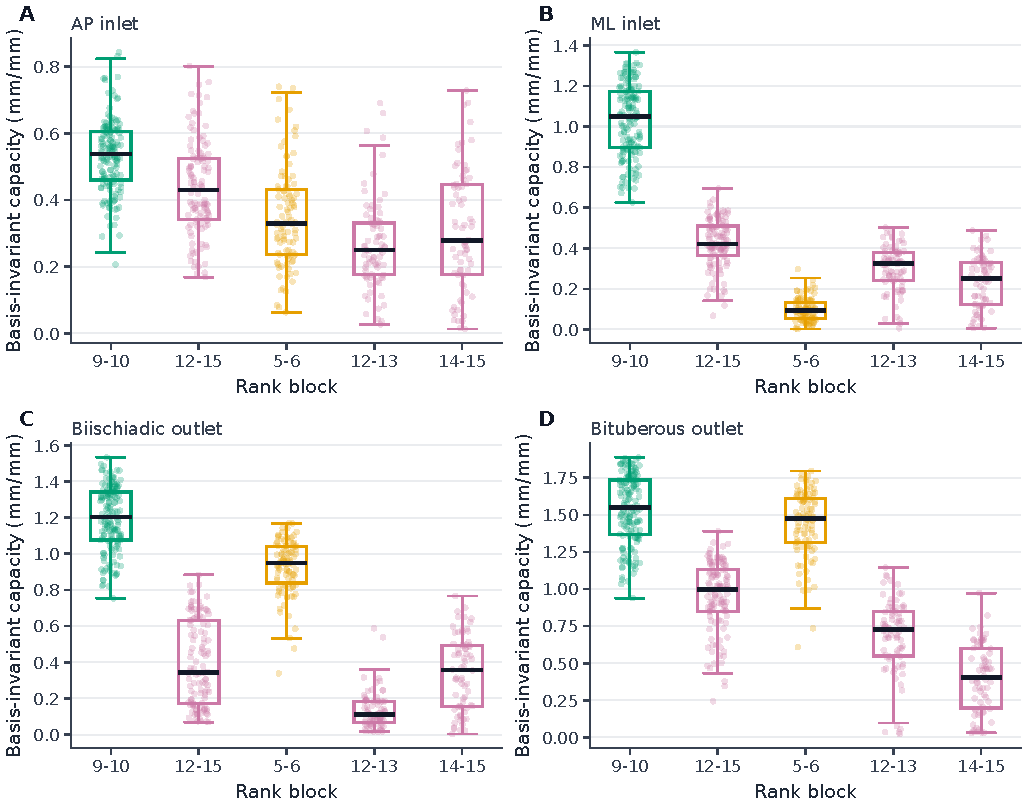
\includegraphics[width=\textwidth]{Fig3.pdf}
  \caption{\textbf{Basis-invariant anatomical capacities across recurrent clustered modal subspaces.}
  Basis-invariant anatomical capacities (maximum anatomical diameter response per 1\,mm maximum nodal displacement) for the five most prevalent rank blocks across the cohort ($N{=}278$):
  \textbf{(A)}~anteroposterior (AP) inlet,
  \textbf{(B)}~mediolateral (ML) inlet,
  \textbf{(C)}~interspinous midpelvic diameter, and
  \textbf{(D)}~bituberous outlet.
  Boxes indicate median and interquartile range (IQR); whiskers extend to $1.5\times\mathrm{IQR}$.}
  \label{fig:subspace-dashboard}
\end{figure}

\subsection{Subspace capacity varies less than individual-rank coupling}
\label{sec:label-results}

The empirical question is whether anatomical capacity differs less between exchange groups when evaluated over a subspace than at an individual rank.
This hypothesis was tested for the most prevalent cluster, rank modes~9--10 (Fig.~\ref{fig:label-stability}).

Among the \ClusterMemberN\ cluster members, \ClusterNoSwapN\ showed no exchange and \ClusterSwapN\ showed exchange. Median AP-inlet coupling at rank 9 decreased from \RankNineNo\ to \RankNineYes\,mm/mm (difference \RankNineDifference; 95\% confidence interval [\RankNineLow, \RankNineHigh]; $p=\RankNinePformatted$), whereas rank-10 coupling increased from \RankTenNo\ to \RankTenYes\,mm/mm ($p=\RankTenPformatted$). Thus, the anatomical response redistributed between neighbouring ranks.

The corresponding subspace capacity changed from \ScalarAPNo\ to \ScalarAPYes\,mm/mm (difference \ScalarAPDifference; 95\% confidence interval [\ScalarAPLow, \ScalarAPHigh]; rank-biserial correlation \ScalarAPRankBiserial). This is approximately a 5\% median decrease, compared with approximately 69\% at rank 9. The difference is smaller, but capacity is not identical between groups: the Mann--Whitney test gives $p=\ScalarAPPformatted$ (Benjamini--Hochberg-adjusted $q=0.040$). The test assesses distributions, whereas the bootstrap interval concerns the median difference; these summaries need not give identical significance conclusions.

Across all \CohortN\ subjects, irrespective of cluster membership, subspace capacity differed by \CohortScalarAPDifference\,mm/mm (95\% confidence interval [\CohortScalarAPLow, \CohortScalarAPHigh]; $p=\CohortScalarAPPformatted$), while rank-level coupling again redistributed strongly. This supports relative stability of the subspace descriptor, without establishing equivalence. Full estimates, effect sizes, joint-SVD comparisons, and adjusted probabilities are provided in Tables~\ref{tab:detail-B3}--\ref{tab:detail-B4}.

Load routing reinforces the same conclusion (Fig.~\ref{fig:si-routing}).
The 9--10 exchange accompanies a large change in rank-level coupling and a smaller change in subspace capacity.
Subspace rotation and the internal 9--10 gap vary across subjects, AP coupling shifts modestly with swap status, and the throughput of the 9--10 block under \LAB\ depends on morphology in a load-specific way.
For \LABone, block throughput decreases with larger AP inlet diameter ($\rho_s{=}{-}0.48$, $p{=}4.3\times10^{-17}$), whereas \LABtwo\ and \LABthree\ show weaker and differently signed trends.
These patterns support the interpretation that inlet-related mechanics remains associated with the 9--10 subspace even as anatomical variability redistributes its basis representation and modulates its load-specific amplitude.

\begin{figure}[!t]
  \centering
  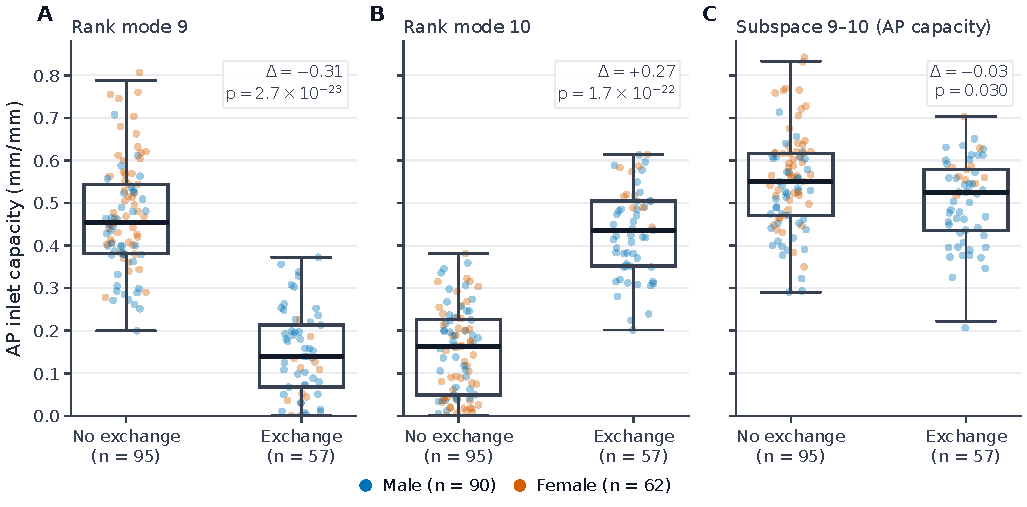
\includegraphics[width=\textwidth]{Fig4.pdf}
  \caption{\textbf{Inlet coupling redistributes between rank labels within the stable 9--10 subspace.}
  Anteroposterior (AP) inlet coupling for rank mode~9 \textbf{(A)}, rank mode~10 \textbf{(B)}, and the basis-invariant single-functional AP capacity of the two-dimensional 9--10 subspace \textbf{(C)}, stratified by $9\rightleftarrows 10$ label-exchange status.
  Points represent individual cluster-member subjects ($n{=}\ClusterMemberN$; no-exchange $n{=}\ClusterNoSwapN$, exchange $n{=}\ClusterSwapN$; male in blue, $n{=}\ClusterMaleN$; female in yellow, $n{=}\ClusterFemaleN$).
  Horizontal lines indicate medians; boxes indicate interquartile range; whiskers indicate $1.5\times\mathrm{IQR}$.
  Coupling is expressed as diameter change per millimetre of maximum nodal displacement.}
  \label{fig:label-stability}
\end{figure}




\FloatBarrier
\subsection{Cohort robustness and sex effects}\label{sec:details-B}

The analysis reports exploratory sex-group comparisons where they help describe variation of the recurrent clustered subspaces, especially the 9--10 inlet-related pair.
This analysis provides the broader sex-stratified summary and the bootstrap stability evidence that the dominant clusters are stable cohort-level features rather than products of a few outlying subjects.
Table~\ref{tab:detail-B1} gives the bootstrap stability estimates (500 replicates of 80\% cohort size drawn with replacement, $m = 222$) for the dominant clusters and gap statistics.
Fig.~\ref{fig:detail-B1} summarises the sex-stratified spectral structure, and Table~\ref{tab:detail-B2} reports the accompanying sex-stratified statistical tests for the spectral and subspace metrics.

\begin{table*}[!htbp]
\caption{Cohort bootstrap stability under random 80\% fractional resamples ($m=222$, 500 replicates with replacement). }
\label{tab:detail-B1}
\centering
\DetailTableInput{cohort_bootstrap_robustness.tex}
\end{table*}


\begin{figure}[!htbp]
\centering

  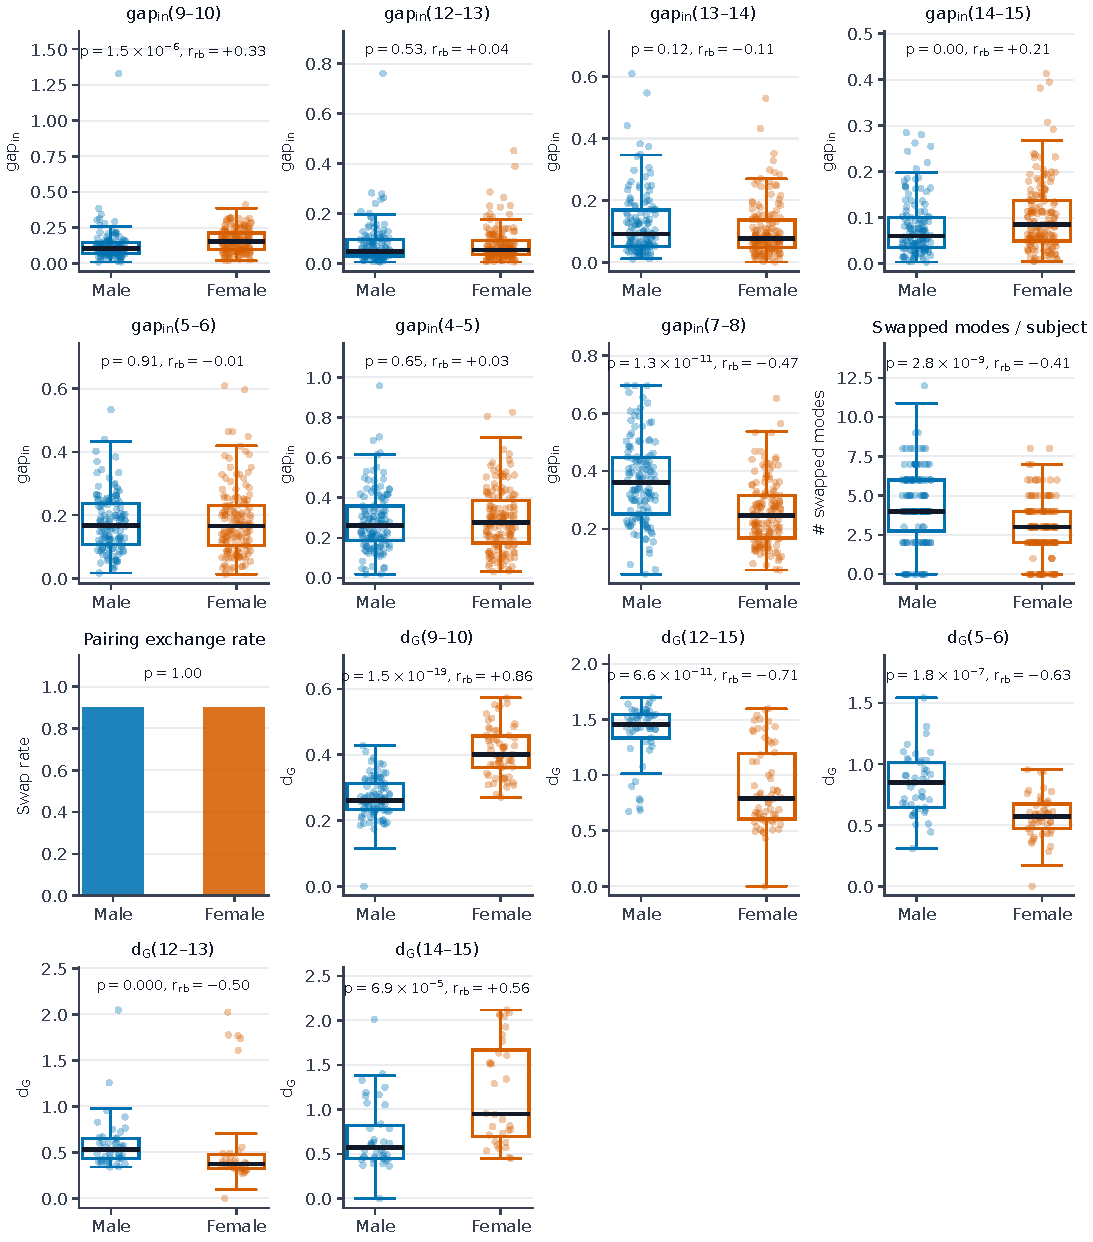
\includegraphics[width=\linewidth]{sex_stratified_summary.pdf}

\caption{Sex-stratified spectral summary}
\label{fig:detail-B1}
\end{figure}


\begin{table*}[!htbp]
\caption{Exploratory sex-stratified tests. Probabilities are unadjusted. Subspace distances use cluster-member subjects; other rows use the full cohort. The permutation-rate row reports a Fisher test, whose statistic is an odds ratio rather than Mann--Whitney $U$. }
\label{tab:detail-B2}
\centering
\DetailTableInput{sex_stratified_summary.tex}
\end{table*}




\begin{table*}[!htbp]
\caption{Cluster members: rank and subspace comparisons. No exchange: $n=95$; exchange: $n=57$. Couplings and differences are in mm/mm. Difference is exchange minus no exchange; intervals use 5,000 percentile bootstrap resamples. $p$ is the two-sided Mann--Whitney probability, $q$ its Benjamini--Hochberg adjustment across the four metrics in this table, and $r_{\rm rb}$ the rank-biserial effect. The joint-SVD score is distinct from single-functional capacity.}
\label{tab:detail-B3}
\centering
\DetailTableInput{label_effects_compact.tex}
\end{table*}


\begin{table*}[!htbp]
\caption{Full cohort, irrespective of cluster membership: rank and subspace comparisons. No exchange: $n=204$; exchange: $n=74$. Couplings and differences are in mm/mm. Difference is exchange minus no exchange; intervals use 5,000 percentile bootstrap resamples. $p$ is the two-sided Mann--Whitney probability, $q$ its Benjamini--Hochberg adjustment across the four metrics in this table, and $r_{\rm rb}$ the rank-biserial effect. The joint-SVD score is distinct from single-functional capacity.}
\label{tab:detail-B4}
\centering
\DetailTableInput{label_effects_full_cohort_compact.tex}
\end{table*}




\FloatBarrier
\subsection{Standing and proxy loads distinguish backbone-dominated routing from higher-rank recruitment}
\label{sec:load-results}

Load routing reflects the same separation between conserved baseline support and selective higher-rank recruitment (Fig.~\ref{fig:fractions-panel}, Table~\ref{tab:dominant-sets}).
Standing is dominated by the gap-protected low-rank backbone.
Symmetric two-leg standing (SP2leg) is concentrated in mode~2 alone, which carries about 84.5\% of the retained modal strain energy; single-leg standing (SP1leg) distributes energy across the full rotational triad (modes~1--3), reaching a top-3 cumulative share of about 92.0\%.
Under these two prescribed standing loads, a few low-rank modes account for most of the retained modal energy.

The proxy load family recruits higher-rank modes.
\LABone, bilateral mediolateral internal ring expansion ($\pm 400$\,N outward), preferentially engages the rank~9--10 inlet-related subspace, which carries a mean energy share of about 0.51 and is led by the inlet-opening mode.
\LABtwo, bilateral ischial-tuberosity distraction, reroutes energy into the mid-rank block at modes~4--8, where the 5--6 outlet-related pair becomes especially important.
\LABthree, anteroposterior outlet distraction, is hybrid, retaining sizeable low-rank contributions while also recruiting mid-rank and 9--10 pathways.
Different loading geometries recruit different parts of the higher-rank spectrum, while continuing to use the backbone as common support.

Among the recurrent clustered regimes, 9--10 remains the clearest case because it combines high cohort prevalence, clear inlet-related interpretation, direct label-versus-subspace evidence (Fig.~\ref{fig:label-stability}), and substantial recruitment under \LABone.
The 5--6 pair remains an outlet-related secondary contrast under \LABtwo, whereas 12--15 is common but behaves, under the present load family, as a mixed higher-rank reserve rather than a single dominant pathway.
Primary cohort routing is evaluated on the total static response. Archived incremental outputs for 18 subjects showed unchanged top-mode identity across all five loads, but individual 9--10 block fractions shifted by up to 4.24 percentage points and dominant-set size changed in four \LABone\ cases (Section~\ref{sec:loading}).
Additional load-specificity and sex-stratified summaries are reported in Section~\ref{sec:details-B} and Section~\ref{sec:details-C}.

These are linear comparative proxy loads, not simulations of labour.
They do not model fetal contact, tissue remodelling, hormone-dependent softening, or nonlinear late-stage birth mechanics.
Their value is comparative: they reveal which deformation patterns are preferentially recruited under different loading geometries, not whether the model can predict clinical childbirth outcomes.

\begin{figure}[!t]
  \centering
  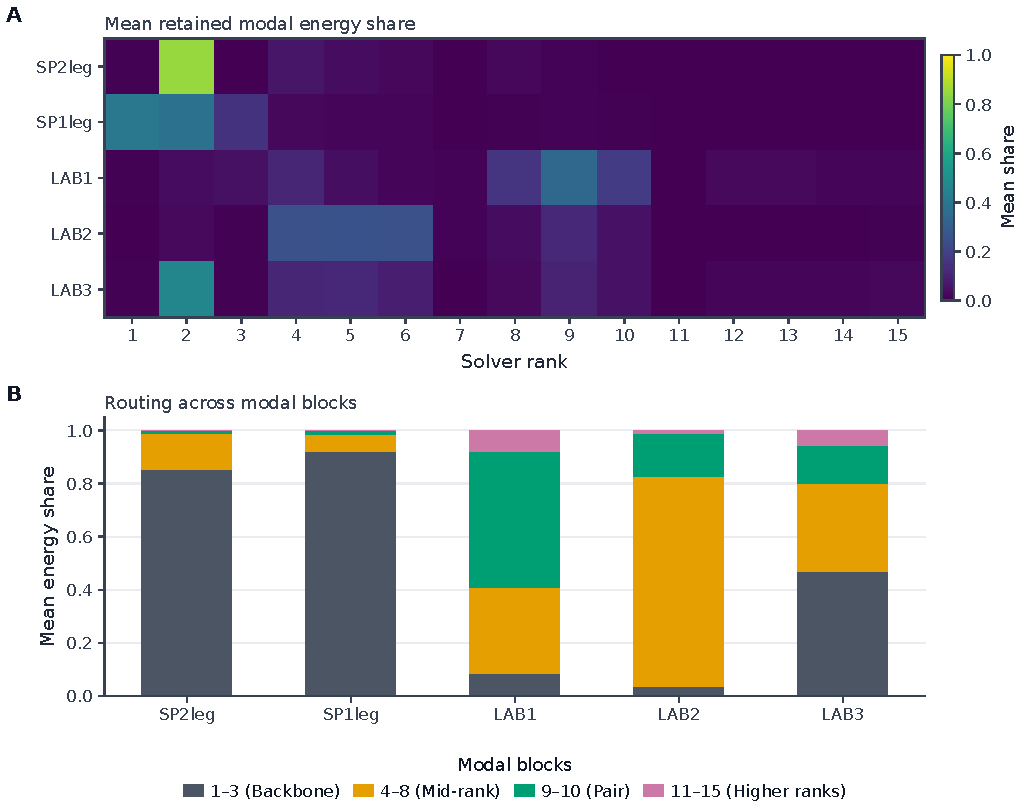
\includegraphics[width=\textwidth]{Fig5.pdf}
  \caption{\textbf{Standing and proxy childbirth loads recruit distinct modal regimes.}
  \textbf{(A)} Heatmap of mean retained modal strain-energy share across the 15 lowest solver ranks for standing (SP2leg, SP1leg) and proxy childbirth loads (\LABone--\LABthree).
  \textbf{(B)} Partition of retained modal strain energy across functional blocks: low-rank backbone (modes~1--3; blue), mid-rank regime (modes~4--8; orange), inlet cluster (modes~9--10; green), and higher-rank reserve (modes~11--15; purple). Standing concentrates in the backbone, whereas proxy loads recruit higher ranks in a task-specific pattern.}
  \label{fig:fractions-panel}
\end{figure}

\begin{table*}[!t]
\centering
\caption{\textbf{Dominant mode sets for the standing and proxy loading cases.}
$N_{80}$ denotes the smallest set of modes required to reach 80\% cumulative mean energy fraction.}
\label{tab:dominant-sets}
\StdTableFont
\StdTableInput{mode_activation_dominant_sets.tex}
\end{table*}


\FloatBarrier
\subsection{Load-routing specificity}\label{sec:details-C}

The study uses standing and proxy childbirth loads to show the contrast between a robust low-rank backbone and selectively recruited higher-rank subspaces.
This analysis provides comprehensive load-specificity diagnostics, including cluster-level function-locking, dominant-mode sets, and pairwise overlap of full routing profiles.

Fig.~\ref{fig:detail-C1} visualises the load--function locking map across the prevalent clusters.
Table~\ref{tab:detail-C1} summarises the phase-specific coupling synthesis, Table~\ref{tab:dominant-sets} summarises the dominant mode sets, and Table~\ref{tab:detail-C3} reports the pairwise overlap metrics for the full load-routing profiles.

\begin{figure}[!htbp]
\centering

  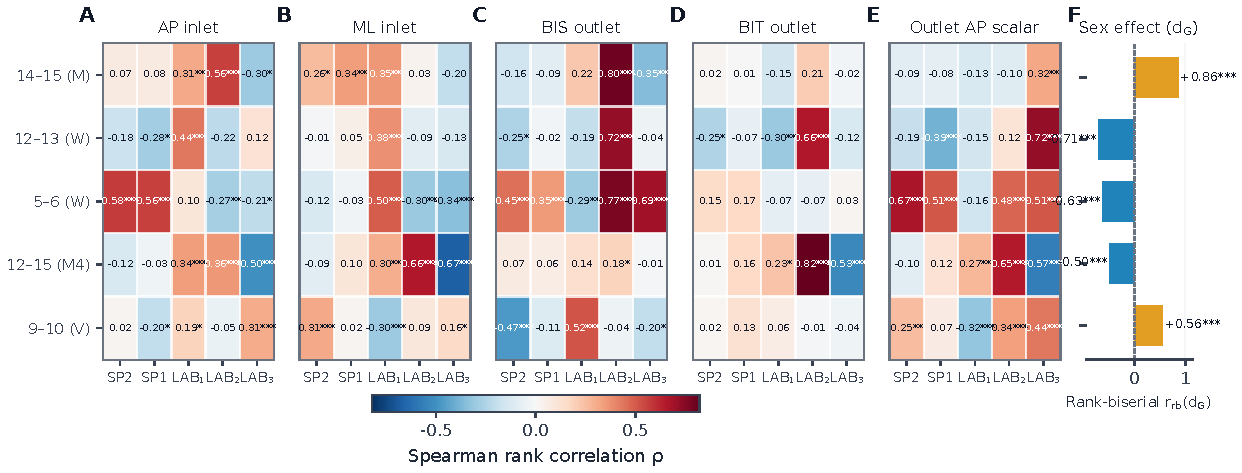
\includegraphics[width=\linewidth]{function_locking_heatmap.pdf}

\caption{Load-function coupling heatmap across prevalent clusters}
\label{fig:detail-C1}
\end{figure}


\begin{table*}[!htbp]
\caption{Exploratory load--coupling associations among cluster members. AP/ML and BIS/BIT scores are earlier paired-SVD descriptors; Outlet AP uses an $L^2$-optimal direction followed by max-nodal normalisation. These differ from the max-nodal capacity in the main comparison. FLI selects the strongest Spearman association among five axes and is descriptive. The energy column is the within-cluster median. }
\label{tab:detail-C1}
\centering
\DetailTableInput{function_locking_synthesis.tex}
\end{table*}




\begin{table*}[!htbp]
\caption{Pairwise overlap of load-routing profiles. }
\label{tab:detail-C3}
\centering
\DetailTableInput{mode_activation_overlap.tex}
\end{table*}



\begin{figure}[!htbp]
  \centering
  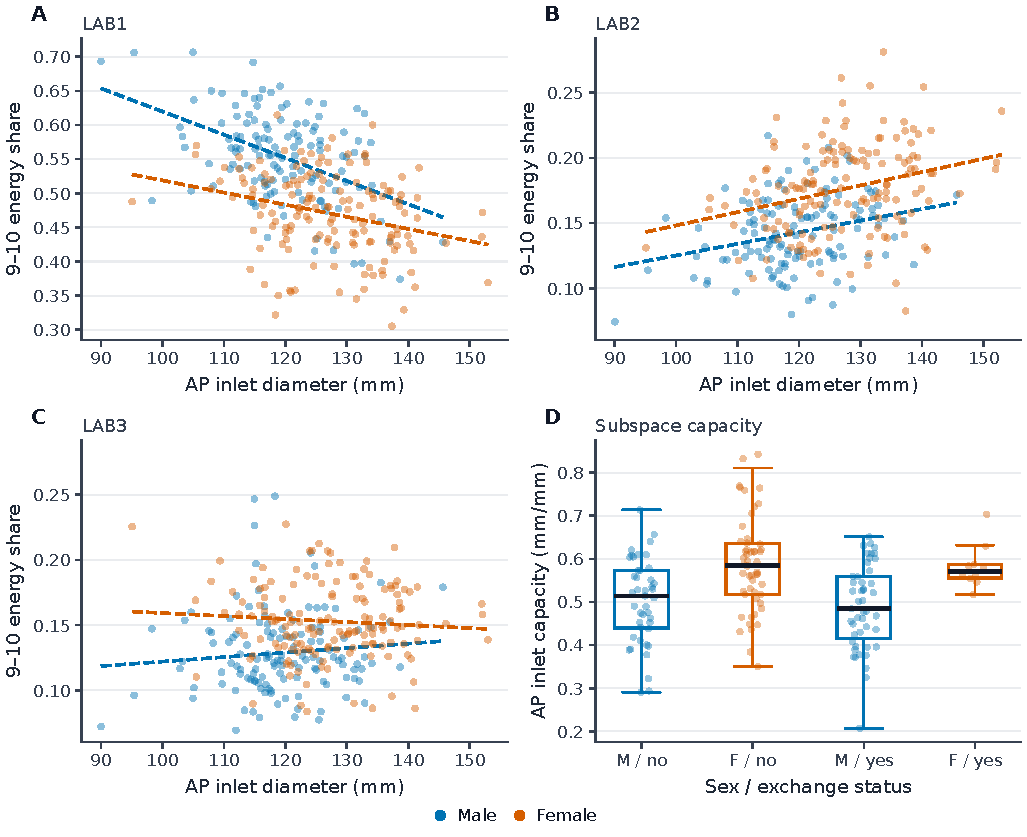
\includegraphics[width=\linewidth]{routing_associations.pdf}
  \caption{\textbf{Morphology and loading modulate recruitment of the 9--10 modal block.}
  \textbf{(A--C)} Modal strain-energy fraction carried by the 9--10 block as a function of AP inlet diameter for \LABone\ (bilateral internal ring expansion), \LABtwo\ (ischial distraction), and \LABthree\ (outlet distraction).
  Blue dots and dashed lines indicate males; yellow dots and dashed lines indicate females.
  \textbf{(D)} Basis-invariant single-functional AP-inlet capacity of the 9--10 subspace stratified jointly by sex and label-exchange status (M/no, F/no, M/yes, F/yes). Boxes show median and IQR; whiskers extend to $1.5\times\mathrm{IQR}$.}
  \label{fig:si-routing}
\end{figure}


\FloatBarrier
\subsection{First-order material sensitivity differentiates spectral regions}\label{sec:uq-results}
First-order propagation with derivatives of the implemented material map predicts substantial variation in absolute eigenvalues under the assumed covariance; shared-parameter covariance reduces the calculated uncertainty of adjacent differences (Fig.~\ref{fig:material-uq}; Table~\ref{tab:detail-D2}). Mean gap signal-to-noise ratios exceed 2 for ranks 1--2 and 2--3 in both sexes, whereas the 9--10 mean is 0.997 in females and 0.947 in males. Under this assumed local perturbation model, the internal 9--10 ordering is therefore more susceptible than the low-rank gaps. The calculation concerns eigenvalues and gaps; it does not independently verify preservation of subspace orientation or anatomical capacity under large material changes.

\begin{figure}[!t]
  \centering
  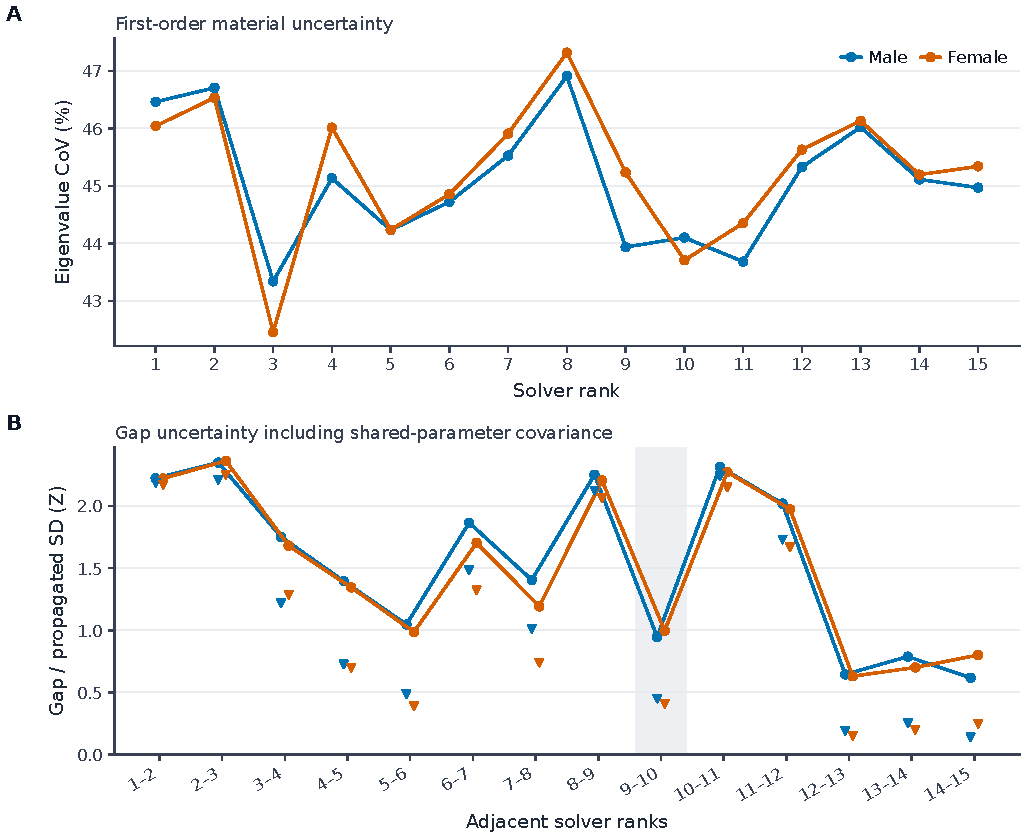
\includegraphics[width=\textwidth]{Fig6.pdf}
  \caption{\textbf{Analytical propagation of material-parameter uncertainty to eigenvalues and spectral gaps.}
  \textbf{(A)} Total coefficient of variation (CoV, \%) of eigenvalues $\lambda_1,\ldots,\lambda_{15}$ under hierarchical material-parameter covariance, stratified by sex (blue: male; yellow: female).
  \textbf{(B)} Relative gap signal-to-noise ratio (spectral gap divided by propagated standard deviation) between adjacent solver ranks, incorporating shared-parameter covariance $\mathrm{Cov}(\lambda_i, \lambda_{i+1})$.
  The shaded region highlights the 9--10 rank transition. Triangles mark 10th-percentile values across subjects.}
  \label{fig:material-uq}
\end{figure}
\FloatBarrier
\subsection{Model-boundary and sensitivity analyses}\label{sec:details-D}

These analyses bound the main claims rather than extend them.
Allometry describes associations between the archived spectra and isotropic size; it is not a recovery of information proven to have been removed by geometric normalisation.
The corrected material-uncertainty calculation illustrates how assumed soft-tissue and density-law scatter could affect eigenvalues and spectral gaps to first order.
Fig.~\ref{fig:detail-D1} shows the post-hoc allometric recovery analysis, and Table~\ref{tab:detail-D1} summarises the corresponding scaling exponents and variance decomposition.
Fig.~\ref{fig:detail-D2} presents the threshold sensitivity, reference sensitivity, isotropic scale vs solver gap, and 15-mode displacement reconstruction error (tabulated in Table~\ref{tab:detail-D3}), alongside Table~\ref{tab:detail-D2} which tabulates the combined first-order uncertainty propagation used to support the robustness discussion in the article.

\begin{figure}[!htbp]
\centering

  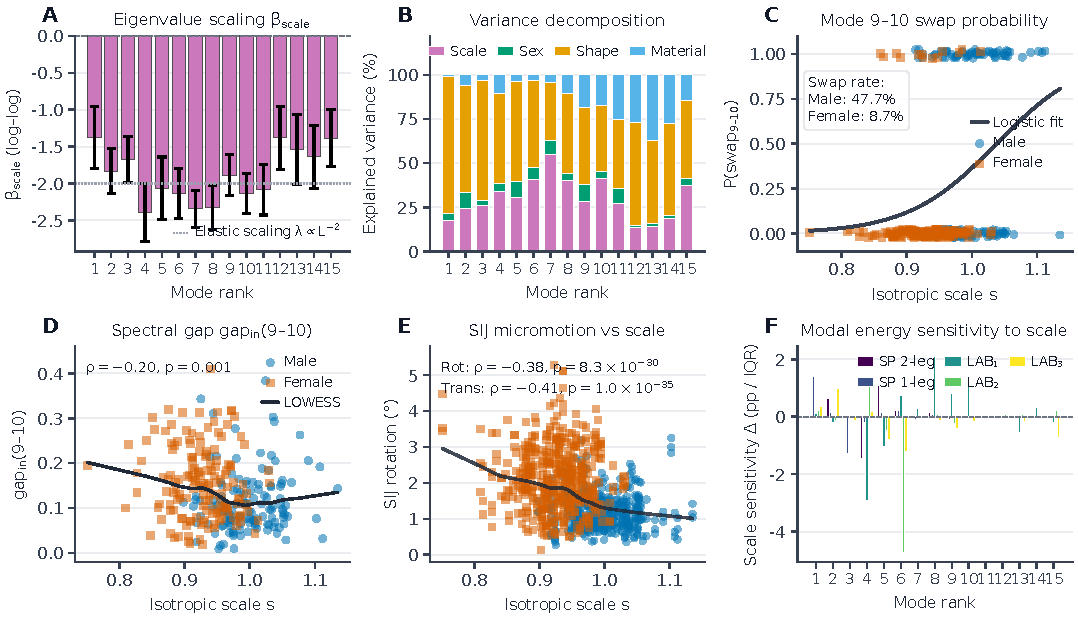
\includegraphics[width=\linewidth]{allometry_dashboard.pdf}

\caption{Allometry dashboard}
\label{fig:detail-D1}
\end{figure}




\begin{table*}[!htbp]

\centering
\caption{Allometric scaling exponents and variance decomposition per eigenvalue mode. $\beta_{\rm scale}$ is the IV-2SLS log--log coefficient of eigenvalue on isotropic scale, with HC-robust 95\,\% CIs and FDR-corrected $p$-values. $\Delta\lambda$ per IQR gives the percent eigenvalue change for an interquartile range shift in log-scale. The last four columns show LMG (Shapley) shares of explained variance divided by full-model $R^2$; they sum to approximately 100\% and are not percentages of total outcome variance. These are descriptive associations, not identified causal effects.}
\label{tab:detail-D1}
\small
\resizebox{\linewidth}{!}{%
\begin{tabular}{ccccccccc}
\toprule
Mode & $\beta_{\rm scale}$ & 95\% CI & $p_{\rm FDR}$ & $\Delta\lambda$ IQR (\%) & R$^2$ scale (\%) & R$^2$ shape (\%) & R$^2$ material (\%) & R$^2$ sex (\%) \\
\midrule
1 & -1.38 & [-1.80, -0.96] & 4.7e-10 & -10.1 & 17.4 & 77.5 & 1.1 & 3.9 \\
2 & -1.83 & [-2.14, -1.53] & 8.4e-26 & -13.1 & 24.2 & 60.6 & 5.8 & 9.4 \\
3 & -1.68 & [-1.99, -1.36] & 2.0e-21 & -12.1 & 26.2 & 68.0 & 3.1 & 2.7 \\
4 & -2.39 & [-2.78, -2.00] & 7.7e-27 & -16.8 & 33.9 & 50.8 & 10.9 & 4.4 \\
5 & -2.07 & [-2.49, -1.64] & 1.1e-18 & -14.7 & 30.4 & 56.8 & 3.6 & 9.3 \\
6 & -2.14 & [-2.48, -1.80] & 3.4e-28 & -15.1 & 40.7 & 48.8 & 3.5 & 7.1 \\
7 & -2.35 & [-2.60, -2.10] & 5.7e-49 & -16.5 & 54.8 & 33.1 & 4.3 & 7.8 \\
8 & -2.33 & [-2.63, -2.02] & 2.4e-37 & -16.4 & 40.2 & 45.3 & 10.4 & 4.1 \\
9 & -1.89 & [-2.16, -1.61] & 1.9e-31 & -13.5 & 28.5 & 43.8 & 18.3 & 9.4 \\
10 & -2.14 & [-2.41, -1.87] & 7.7e-39 & -15.1 & 41.5 & 37.4 & 17.4 & 3.7 \\
11 & -2.09 & [-2.43, -1.75] & 6.3e-27 & -14.8 & 27.0 & 39.1 & 25.4 & 8.5 \\
12 & -1.38 & [-1.81, -0.95] & 9.4e-10 & -10.1 & 13.5 & 58.1 & 27.1 & 1.3 \\
13 & -1.54 & [-2.02, -1.07] & 8.2e-10 & -11.2 & 14.1 & 47.0 & 37.4 & 1.5 \\
14 & -1.64 & [-2.07, -1.21] & 1.5e-12 & -11.8 & 18.5 & 52.2 & 27.4 & 1.9 \\
15 & -1.39 & [-1.77, -1.00] & 1.8e-11 & -10.1 & 37.4 & 43.8 & 14.8 & 3.9 \\
\bottomrule
\end{tabular}%
}


\end{table*}




\begin{figure}[!htbp]
\centering

  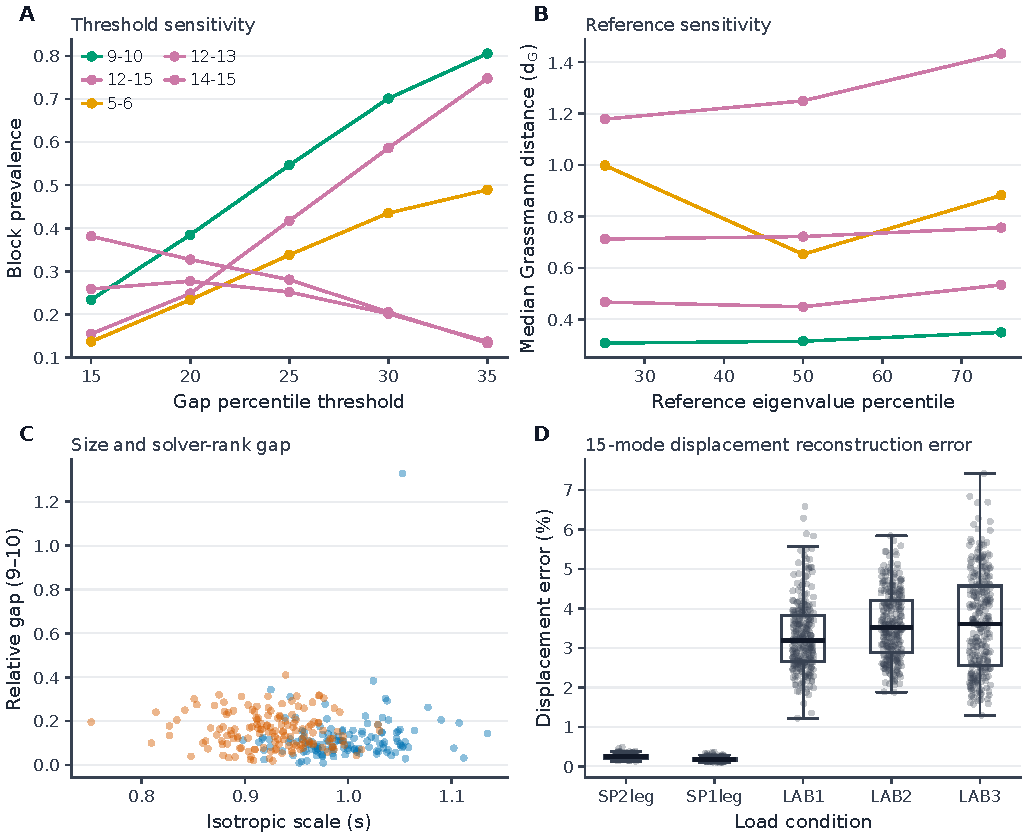
\includegraphics[width=\linewidth]{robustness.pdf}

\caption{Robustness and reconstruction dashboard}
\label{fig:detail-D2}
\end{figure}




\begin{table*}[!htbp]

\centering
\small
\caption{Population-level material uncertainty propagation stratified by sex. CoV is the total coefficient of variation (ligament + cartilage + bone). Lig/Cart/Bone columns show each group's fraction of total variance. The bone contribution uses derivatives of the implemented density-to-modulus map. Gap signal-to-noise ratios are displayed in Fig.~\ref{fig:material-uq}, not in this table.}
\label{tab:detail-D2}
\begin{tabular}{l cccc cccc}
\toprule
& \multicolumn{4}{c}{Female ($N=150$)} & \multicolumn{4}{c}{Male ($N=128$)} \\
\cmidrule(lr){2-5} \cmidrule(lr){6-9}
Mode & CoV & Lig & Cart & Bone & CoV & Lig & Cart & Bone \\
     & (\%) & (\%) & (\%) & (\%) & (\%) & (\%) & (\%) & (\%) \\
\midrule
1 & 46.0 & 5 & 94 & 0 & 46.5 & 7 & 93 & 0 \\
2 & 46.5 & 4 & 93 & 2 & 46.7 & 5 & 93 & 2 \\
3 & 42.5 & 5 & 94 & 1 & 43.3 & 6 & 93 & 1 \\
4 & 46.0 & 6 & 90 & 4 & 45.1 & 8 & 90 & 2 \\
5 & 44.2 & 8 & 89 & 3 & 44.2 & 9 & 89 & 2 \\
6 & 44.9 & 9 & 89 & 2 & 44.7 & 10 & 88 & 2 \\
7 & 45.9 & 16 & 83 & 1 & 45.5 & 15 & 84 & 1 \\
8 & 47.3 & 7 & 90 & 3 & 46.9 & 6 & 91 & 3 \\
9 & 45.2 & 4 & 88 & 7 & 43.9 & 4 & 90 & 5 \\
10 & 43.7 & 2 & 90 & 8 & 44.1 & 5 & 90 & 6 \\
11 & 44.4 & 1 & 87 & 11 & 43.7 & 3 & 89 & 9 \\
12 & 45.6 & 1 & 86 & 14 & 45.3 & 2 & 85 & 13 \\
13 & 46.1 & 1 & 84 & 15 & 46.0 & 1 & 83 & 16 \\
14 & 45.2 & 1 & 86 & 13 & 45.1 & 2 & 88 & 10 \\
15 & 45.3 & 2 & 88 & 9 & 45.0 & 3 & 89 & 8 \\
\bottomrule
\end{tabular}


\end{table*}



\begin{table*}[!htbp]
\caption{Relative displacement reconstruction error for 15 modes. Errors are relative displacement norms, expressed as fractions rather than percentages. These are displacement diagnostics and do not establish strain-energy or local stress accuracy.}
\label{tab:detail-D3}
\centering
\DetailTableInput{reconstruction.tex}
\end{table*}



\FloatBarrier
\subsection{A three-coordinate model illustrates label--subspace dissociation}
\label{sec:toy-results}

The constructed analytical example illustrates how a separated low-rank mode and a coupled higher pair can produce contrasting rank and subspace behaviour (Fig.~\ref{fig:toy}). As detuning varies, the dominant projection of the anatomical observable transfers between the upper eigenvectors, whereas their summed projection remains high. Standing-like and task-like loads recruit different spectral regions. Increasing the nuisance scale changes the dominant carrier more strongly than the upper-pair projection or task routing.

The example conditions accepted draws on a retained low-rank backbone. Its observable is a squared projection, rather than the max-nodal capacity used in the pelvic analysis. It therefore illustrates a spectral mechanism without independently establishing either pelvic rank stability or tissue-specific compensation. The cohort permutation test did not detect exchange localisation along AP inlet diameter alone (Table~\ref{tab:detail-A6}; all tested cases $p>0.05$). A single anatomical coordinate is consequently not supported as an explanation of the observed exchange.

\begin{figure}[!t]
  \centering
  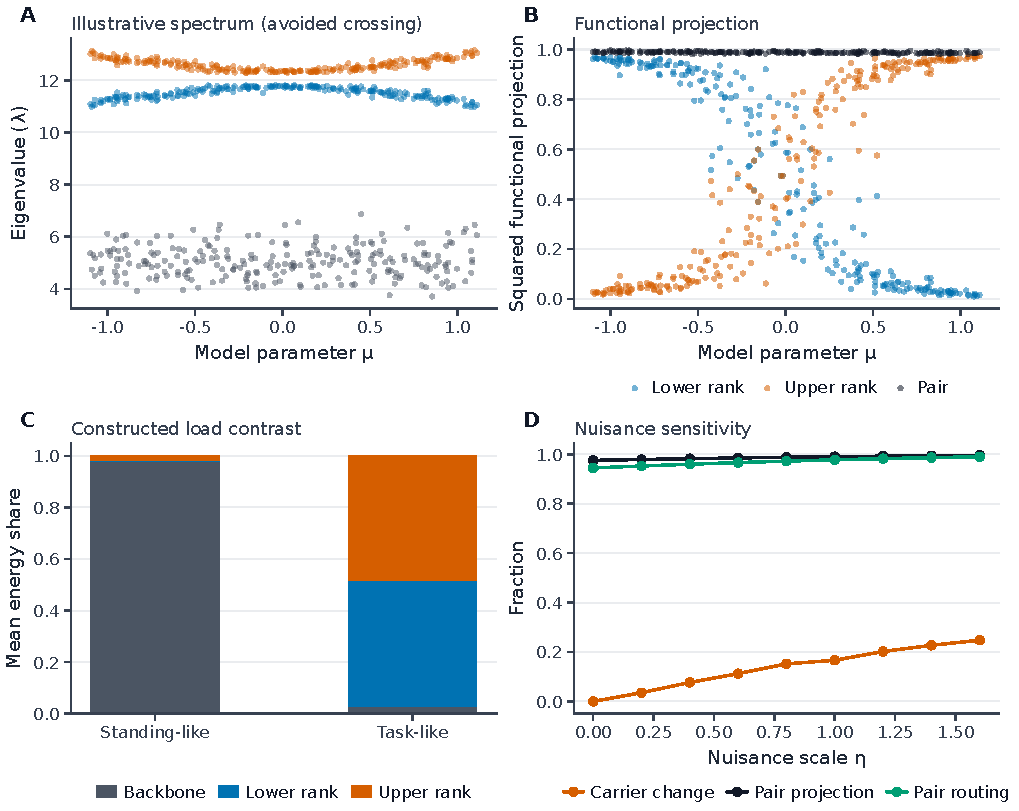
\includegraphics[width=\textwidth]{Fig7.pdf}
  \caption{\textbf{Minimal analytical model illustrates label exchange within a stable subspace.}
  A stochastic cohort of the analytical model with morphology parameter~$\mu$ and hidden-pathway scale~$\eta$.
  \textbf{(A)} Spectrum: a separated backbone mode and a nearby eigenvalue pair undergoing near-degeneracy around $\mu \approx 0$.
  \textbf{(B)} Functional projection: coupling shifts between individual rank labels across the transition zone while total coupling within the pair remains high.
  \textbf{(C)} Load routing: standing-like load concentrates in the backbone, whereas task-like load recruits the clustered block with a variable between-label split.
  \textbf{(D)} Effect of hidden-pathway variability scale~$\eta$: label-exchange rate increases with~$\eta$, whereas subspace coupling and task routing remain stable.
  Model derivations and simulation parameters are detailed in Sections~\ref{sec:toy-methods}--\ref{sec:toy-specification}.}
  \label{fig:toy}
\end{figure}

% ============================================================
\section{Discussion}\label{sec:discussion}
\subsection{The comparative unit depends on spectral separation}
The principal finding is that anatomical coupling can be much less sensitive to cross-subject mode exchange when evaluated over a small subspace than at one fixed eigenvalue rank. Within the recurrent 9--10 cluster, median rank-9 AP-inlet coupling decreases from \RankNineNo\ to \RankNineYes\,mm/mm between non-exchange and exchange groups, approximately 69\%, whereas the corresponding subspace capacity decreases from \ScalarAPNo\ to \ScalarAPYes\,mm/mm, approximately 5\%. This difference matters for population biomechanics: interpreting rank 9 alone as a conserved inlet-opening pathway would overstate the change in that block's kinematic capacity.

The result combines three distinct measurements. Modal assignment identifies changes in correspondence to a reference; principal angles quantify changes in subspace orientation; and anatomical functionals evaluate specific diameter responses. Basis invariance alone guarantees independence from the chosen coordinates within a fixed subspace, not stability across anatomically different subjects. Cross-subject preservation is therefore an empirical question, addressed here by the distribution of anatomical capacities. The observed differences support relative stability, rather than exact conservation or a demonstrated equivalence between exchange groups.

This interpretation applies selectively across the spectrum. Modes 1--3 retain their ordering in almost all subjects, making individual-mode comparison comparatively well conditioned. Higher ranks contain recurrent small-gap blocks. The 9--10 block is the clearest interior example; the 12--15 block remains incompletely characterised because its upper spectral neighbour was not computed. The analysis consequently supports choosing comparison units using both internal gaps and external separation, rather than grouping all higher modes indiscriminately.

\subsection{Anatomical capacity and load recruitment answer different questions}
Anatomical capacity estimates the largest diameter change within a subspace at a specified displacement normalisation; the two-dimensional estimates were spot-checked against a constrained solver. It does not measure deformation per unit force and does not predict how strongly that subspace is recruited by a particular load. Static modal energy provides the complementary load-dependent quantity. Standing mainly recruits low ranks, whereas internal-ring expansion increases recruitment of the 9--10 block. The 5--6 pair is relevant to ischial distraction despite not having the largest outlet capacity among the compared blocks.

These findings provide a mechanical description of the initial deformation repertoire of a constrained pelvic ring. They may help formulate hypotheses about how load transfer and canal deformation coexist, a longstanding question in pelvic biomechanics~\citep{Gruss2015}. They do not demonstrate evolutionary optimisation, physiological compensation, or birth-canal expansion during actual labour. In particular, the mixed-sex cohort and its mean age of approximately 54 years limit direct inference to pregnant or primiparous populations. The minimal analytical example illustrates the spectral mechanism and was constructed to retain the backbone; it is not an independently validated physiological model.

\subsection{Implications for population finite-element studies}
The present analysis extends the pelvic eigenmetric approach of \citet{Henys2021Eigenmetric} from spectral descriptors toward the correspondence of anatomically meaningful deformation spaces across subjects. Its distinction from load-specific cohort analyses, such as the strain comparisons of \citet{Salo2017PelvicStrain}, is the separate evaluation of available kinematic capacity and load recruitment. The numerical rationale for following clustered subspaces is established~\citep{GhoshGhanem2012}; the evidence added here is the magnitude of the discrepancy between rank-level and subspace-level anatomical comparisons in a pelvic population. This finding does not invalidate earlier spectral descriptors, but identifies a correspondence check needed when assigning anatomical meaning to a fixed rank.

The practical contribution is a sequence of comparisons that could be evaluated in other anatomically variable structures: identify crowded spectral regions, verify their external separation, compare their subspaces in a shared metric, and evaluate anatomically meaningful observables together with load-dependent recruitment. This extends established subject-specific finite-element modelling by addressing ambiguity in the interpretation of population modal comparisons~\citep{Fernandez2020Population}. It does not require a new constitutive formulation to reveal a consequential limitation of rank-based interpretation.

The exchange groups are defined from eigenvectors also used to evaluate anatomical coupling. The rank-level contrast is consequently descriptive, not an independent causal effect of exchange. A maximum over two modes is at least as large as the capacity of either included mode; that inequality alone does not guarantee a smaller difference between groups.

The generalisable component is the analysis strategy. The observed rank partition depends on the pelvic geometry, restraints, constitutive assumptions, and retained spectral range. Applying the approach elsewhere requires new anatomical functionals and a fresh assessment of gaps and truncation. Likewise, low-dimensional representations useful for describing global ring kinematics need not resolve local strains or stresses adequately. The polynomial deformation atlas is a descriptive check, with explicit residuals, rather than a validation of physiological deformation pathways.

\subsection{Limitations and validation priorities}
The models assume small strains, isotropic bone elasticity, homogeneous joint cartilage, and prescribed ligament properties. The superior sacral restraint and chosen load locations constrain the available deformation repertoire. Subject-specific ligament laxity, pelvic floor support, nonlinear contact, and time-dependent tissue behaviour are not represented. These omissions limit extrapolation to large deformations, altered joint conditions, and childbirth~\citep{Vleeming2012,ChenGrimm2021}.

The superior sacral restraint uses a fixed penalty parameter ($\gamma=10^6$\,N/mm$^3$); the claimed decade sensitivity sweep could not be verified from retained outputs.

The corrected first-order propagation indicates possible local sensitivity of eigenvalues and gaps under the specified covariance. It does not replace re-solving the full model under broad parameter changes, nor does it verify robustness of eigenvectors and capacities in that setting. The reduced analytical example likewise cannot supply evidence about tissue-specific variability that was not measured in the cohort. Future work should test subspace capacities under explicit soft-tissue perturbations and alternative boundary conditions.

Energy fractions refer to the 15 retained modes. Their sum is unity by normalisation and is not evidence that those modes recover the complete static energy. Displacement reconstruction errors are reported separately, but displacement accuracy does not establish accuracy of local stress or strain. An archived expanded-spectrum check on three subjects reproduced the first 15 eigenvalues with maximum relative discrepancy $3.4\times10^{-11}$. In these subjects, energy capture by 15 modes relative to the full assembled quadratic energy was 99.3--99.5\% for standing and 76.5--94.9\% for expansion loads. This does not establish cohort-wide truncation adequacy or the upper separation of the 12--15 block.

Finally, the present evidence establishes computational behaviour within the model family. Experimental measurements of ring displacement under comparable loading would be needed to validate anatomical coupling and recruitment. Robustness to cohort resampling and selected modelling choices strengthens the computational comparison, while leaving that physiological validation open.

\section{Conclusions}
Across 278 pelvic finite-element models, individual low-rank modes retain stable correspondence, whereas higher-rank anatomical coupling can redistribute between neighbouring eigenvalue ranks. For the recurrent 9--10 block, subspace-level inlet capacity varies substantially less with label-exchange status than single-rank coupling. Comparing compact subspaces therefore helps distinguish changes in modal representation from changes in modelled anatomical deformation capacity. The conclusion concerns population comparisons within a linearised model and motivates targeted experimental and modelling tests.

\FloatBarrier
\section*{Statements and Declarations}
\subsection*{Funding}
This research was supported by the Czech Science Foundation, Grant No. 24-10862S.
\subsection*{Competing interests}
The authors declare no competing interests.
\subsection*{Ethics approval and consent to participate}
This study used previously published anonymised imaging-derived data and precomputed models; no new imaging or interventions were performed. According to the BoneDat descriptor, the source study was approved by the Ethics Committee of the University Hospital Hradec Kralove (reference 202411IO3P), with waiver of informed consent~\citep{HenyssKuchar2025BoneDat}.
\subsection*{Consent for publication}
Not applicable; no identifiable individual participant information is presented.
\subsection*{Data availability}
Summary results supporting this study are included in this article. The source anatomical resource is described in BoneDat~\citep{HenyssKuchar2025BoneDat}; access to underlying clinical imaging is governed by the source study. A public archive of the additional subject-level derived outputs has not yet been established.
\subsection*{Code availability}
The study uses custom Python code for model assembly, spectral analysis, and postprocessing. A public archival release of this code has not yet been established.
\subsection*{Author contributions}
P.H., M.K., and N.H. conceptualised the study. P.H. and M.K. developed the computational models and performed the simulations. P.H., M.K., and A.M. analysed the data. P.H., M.K., A.M., and N.H. interpreted the results and contributed to manuscript writing.

\bibliography{references}
\end{document}
